\documentclass[a4paper,fontsize=12pt,headsepline]{scrbook}

\usepackage[ruled,vlined]{algorithm2e}
\usepackage{amsmath}
\usepackage{amssymb}
\usepackage[english]{babel}
\usepackage[maxnames=99]{biblatex}
\usepackage{booktabs}
\usepackage[T1]{fontenc}
\usepackage{graphicx}
\usepackage[pdftex,hidelinks,plainpages=false,pdfpagelabels]{hyperref}
\usepackage[utf8]{inputenc}
% csquotes must be included after inputenc
\usepackage{csquotes}
\usepackage{listings}
\usepackage{multirow}
\usepackage{microtype}
\usepackage{newtxtext}
\usepackage{newtxmath}
% Suppress warning about \float@addtolists
\usepackage{scrhack}
\usepackage[labelformat=simple,format=hang]{subcaption}
\usepackage{tabularx}
\RequirePackage[l2tabu, orthodox]{nag}

% Hyphenations to avoid overfull boxes
\hyphenation{Yo-shi-yu-ki}
\hyphenation{Ya-su-hi-ro}
\hyphenation{Wa-ta-shi-ba}
\hyphenation{Su-su-mu}
\hyphenation{To-shi-yu-ki}
\hyphenation{Shi-mi-zu}

% Suppress warning about multiple PDFs with page group
\pdfsuppresswarningpagegroup=1

% Allow PDF 1.7 documents to be used in \includegraphics
\pdfminorversion=7

\graphicspath{{./img/}}

% Source code
\lstset{%
  language={C},
  basicstyle={\small\ttfamily},%
  identifierstyle={\small\ttfamily},%
  commentstyle={\small\itshape},%
  keywordstyle={\small\bfseries},%
  ndkeywordstyle={\small\ttfamily},%
  stringstyle={\small\ttfamily},%
  frame={tb},%
  breaklines=true,%
  columns=[l]{fullflexible},%
  numbers=none,%
  xrightmargin=0em,%
  xleftmargin=0em,%
  numberstyle={\scriptsize},%
  stepnumber=1,%
  numbersep=1em,%
  lineskip=-0.5ex,%
  mathescape%
}

% Numbering of subfigures
\renewcommand{\thesubfigure}{(\alph{subfigure})}

\addbibresource{references.bib}

\title{Programmable Interconnect Control Adaptive to Communication Pattern \\
of Applications}
\author{Keichi Takahashi}

\renewcommand{\baselinestretch}{1.30}

\begin{document}

\pagenumbering{roman}

\maketitle

\chapter*{List of Publications}

\pagestyle{myheadings}
\markright{}
\chapter*{Summary}

% 背景
Recent breakthroughs in science have significantly benefited from high
performance computing~(HPC). The majority of HPC systems today adopt cluster
architecture to achieve their massive scalable computing performance. A
cluster is a system of computers connected through a high-performance network
referred to as an interconnect. In a cluster, processes running on different
computing nodes work collectively by exchanging data and messages with one
another over the interconnect. Therefore, the communication performance of the
interconnect is critically important in determining the total computing
performance of a cluster.

% 問題
The inter-process communication of an application running on a cluster system
shows a distinctive pattern that originates from the mathematical model,
discretization method and parallelization strategy used in the application.
The design of an interconnect could be highly optimized for a representative
application expected on the target system by taking the communication pattern
of the application into account. However, this design approach is infeasible
and unrealistic when designing a real-world cluster, since many users share a
single HPC system and each user runs various applications. Therefore, in
contrast to the application-dependent communication pattern, the interconnect
is inherently designed in an application-independent manner, assuming a
uniform communication pattern between processes. As a result, an imbalance in
the packet flow in the interconnect can occur under a non-uniform
communication pattern. This imbalance can lead to traffic congestion on a link
in the interconnect, which lowers the throughput of communication and degrades
the total application performance as a result.

% 目的
This dissertation tackles this degradation of application performance by
adapting the control of packet flow in the interconnect to the communication
pattern of applications. Until recently, such dynamic adaptation of the
interconnect control has been deemed infeasible due to the lack of a
networking architecture, technology, or technique that allows flexible and
dynamic reconfiguration. However, the recent emergence of programmable
networking architectures exemplified by Software-Defined Networking~(SDN) has
opened up the possibility to realize such adaptation. This dissertation aims
to overcome this shortcoming of conventional application-independent
interconnects described in the last paragraph, by establishing a programmable
interconnect control that dynamically manages the packet flow in the
interconnect based on the communication pattern of applications.

% 課題
This dissertation tackles the following three challenges to achieve the goal
described above: (1) analyzing the packet flow in the interconnect, (2)
dynamic adaptation of the interconnect control, and (3) coordinating the
execution of application and interconnect control. The first challenge is
required to observe and understand the imbalance of packet flow in the
interconnect to perform an effective adaptation of the interconnect control.
The second challenge is required to mitigate the imbalance of packet flow and
improve the performance of inter-process communication. The third challenge is
required since many real-world applications exhibit time-varying communication
patterns and therefore the interconnect control needs to be performed in
accordance with the execution of an application.

% 提案1
To address the first challenge, Chapter~\ref{sec:ii} proposes PFAnalyzer, a
toolset for analyzing the packet flow in the interconnect. When designing and
implementing an efficient programmable interconnect control, researchers need
to conduct a systematic analysis over many combinations of applications and
interconnects. Since performing such an analysis on a physical cluster is
time-consuming, this research utilizes simulation to facilitate the analysis.
The proposed toolset is a pair of tools: an interconnect simulator
specialized for programmable interconnects, and a profiler to collect
communication pattern from applications. PFSim allows researchers and
designers working on interconnects to investigate congestion in the
interconnect for an arbitrary cluster configuration and a set of communication
patterns extracted by PFProf. In the evaluation, the accuracy of the
simulation results obtained from PFSim is assessed. Furthermore, how
PFAnalyzer can be used to analyze the effect of programmable interconnect
control is demonstrated.

% 提案2
To address the second challenge, Chapter~\ref{sec:iii} proposes a framework to
accelerate MPI collectives by dynamically controlling the packet flow in the
interconnect. Message Passing Interface~(MPI) is a standardized inter-process
communication library widely used to develop parallel distributed
applications for clusters. Out of the communication primitives provided by
MPI, this research focuses on accelerating collective communication because it
consumes a significant fraction of the execution time of applications. The
network programmability provided by Software-Defined Networking is integrated
into MPI collectives in such a way that collectives are able to effectively
utilize the bandwidth of the interconnect. In particular, this research aims
to reduce the execution time of MPI\_Allreduce, which is a frequently used MPI
collective communication in many simulation codes. The speedup of
MPI\_Allreduce when using the proposed collective acceleration framework is
evaluated.

% 提案3
To address the third challenge, Chapter~\ref{sec:iv} proposes UnisonFlow, a
software-defined coordination mechanism that performs interconnect control in
synchronization with the execution of applications. In a real-world
application, the communication pattern changes with the execution of
application. Therefore, a mechanism to coordinate packet flow control and
execution of application is essential. UnisonFlow is a kernel-assisted
mechanism that realizes such coordination in a per-packet basis while
maintaining significantly low overhead. Evaluation verifies that the
interconnect control can be successfully performed in synchronization with the
execution of the application and the overhead imposed by the coordination
mechanismi is small.

Chapter~\ref{sec:v} concludes this dissertation and discusses future works.

\pagestyle{headings}


\tableofcontents
\listoffigures

\newpage
\thispagestyle{empty}

\pagenumbering{arabic}

\chapter{Introduction}

\section{Background}\label{sec:i-background}

\subsection{High Performance Computing}

% HPCとはなにか
Recent advancement in science has significantly benefited from High
Performance Computing~(HPC). Scientists are able to simulate nature on HPC
systems. HPC helps scientists to develop a better understanding of nature and
answer fundamental questions about our surrounding environment by executing
high-resolution computational models of natural phenomena.

% HPCの応用分野
A wide spectrum of science has taken advantage of the massive computing
capability provided by HPC\@. Various phenomena ranging from atomic scale to
cosmological scale intractable to experimentally observe or reproduce are
simulated on HPC systems. For instance, molecular dynamics simulation reveals
the molecular-level structure and property of matter and their interaction.
This knowledge is used to design better drugs and materials. Earthquake and
Tsunami simulation allows us to predict the impact of seismic activities and
prepare for natural disasters. In addition to simulation applications, data
analysis and machine learning applications are also starting to leverage HPC
systems.

% HPCシステムの計算性能の推移
Scientists are trying to tackle increasingly larger and more complex problems.
This continuous demand from domain scientists has kept pushing the performance
HPC systems forward. Figure~\ref{fig:top500-rmax} shows the development of
computing performance of HPC systems based on the data published by the
Top500~\autocite{top500} list. The Top500 list is a biannual list of 500 most
powerful HPC systems measured by the maximal LINPACK benchmark performance
achieved. The plot clearly indicates the exponential increase in performance
over the past 20 years. Researchers and engineers are striving to sustain this
exponential growth in performance and exascale~(Exa FLOPS) in the near future.
To achieve this daunting technological challenge, every aspect of the HPC
system including hardware, operating system, middleware and application need
to be greatly improved, optimized and even redesigned.

\begin{figure}
    \centering
    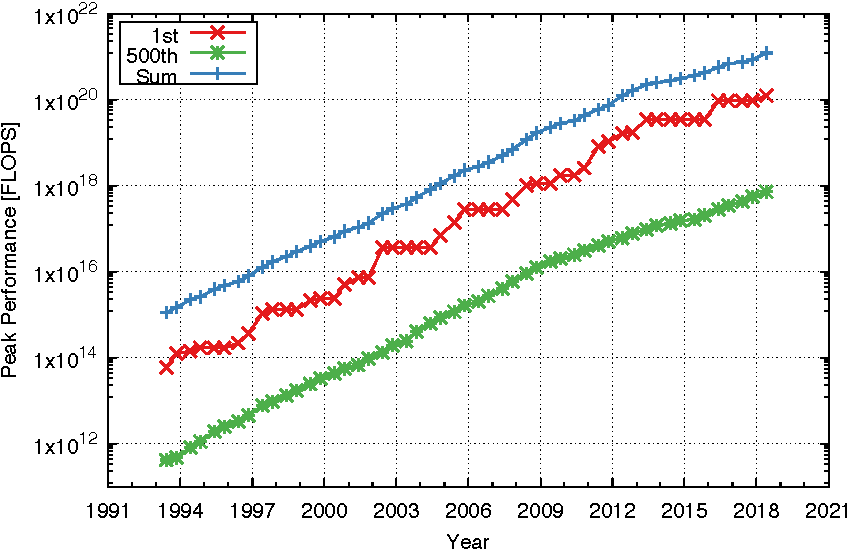
\includegraphics{top500_rmax}
    \caption{Performance Development of Top500 HPC Systems~\autocite{top500}}%
    \label{fig:top500-rmax}
\end{figure}

\subsection{Cluster Architecture}

% クラスタとはなにか
Modern HPC systems mostly adopt \emph{cluster} architecture to achieve their
massive computing performance. In fact, 87\% of the recent Top500 systems
(July 2018) are based on cluster architecture. A cluster is an aggregation of
interconnected computers working cooperatively. Computers that constitute a
cluster perform computation in parallel and exchange data with each other to
required for the computation.

% クラスタの構成要素
Figure~\ref{fig:cluster} shows the architectural overview of a typical
cluster. A cluster consists of multiple computers~(\emph{i.e.,\ computing
nodes}) and a high-performance network that integrates~(\emph{i.e.,\
interconnect}) them together as a single system. Since many users share a
single cluster, a \emph{job scheduler} is deployed to effectively manage the
computing resources in a cluster. A job scheduler accepts jobs from users and
determines when to run each job. The scheduler is also responsible for
allocating computing nodes to a job and launching jobs on allocated nodes.
Furthermore, a shared file systems is usually deployed to store the input and
output data of applications executed on the cluster.

\begin{figure}
    \centering
    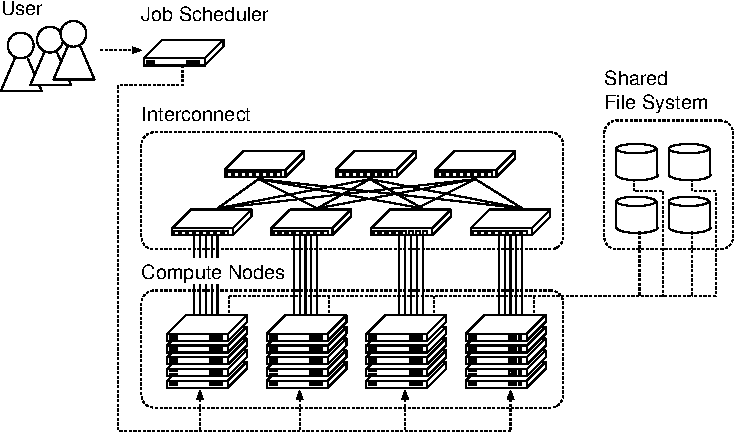
\includegraphics{cluster}
    \caption{Cluster Architecture}%
    \label{fig:cluster}
\end{figure}

% クラスタの規模拡大
There has been an increasing trend in the number of computing nodes that
compose a cluster. Although the computing performance of a single processor
and computing node have been steadily improving, the growth is not fast enough
to meet the high demand for computing power from the users. Therefore, the
designers of HPC systems need to increase the number of computing nodes to
further improve the total computing performance of the cluster. As a result, a
single cluster accommodates up to tens of thousands of computing nodes and
millions of cores nowadays.

% 相互結合網の重要性
The performance of communication between computing nodes over the interconnect
is essential to the scalability of the cluster. In general, computing nodes
need to frequently communicate with each other during the parallel computation
to exchange intermediate results. If the communication between computing nodes
becomes a bottleneck, simply adding more nodes to the cluster does not
increase the total performance of the cluster. Therefore, great effort has
been put to the research and development of high-performance interconnects.

\subsection{Interconnect}\label{sec:i-interconnect}

There are mainly two design goals of a high-performance interconnect: high
bandwidth and low latency.

% 通信規格
Ethernet~\autocite{Trowbridge2007} and InfiniBand~\autocite{Buyya2009} are
network technology standards commonly utilized for interconnects. Ethernet is
a long-standing network technology that has been ubiquitously used in both
local area networks and wide are networks. InfiniBand, on the other hand, is a
network standard specifically designed with HPC in mind. InfiniBand offloads
most of its protocol stack onto hardware and realizes mechanisms such as
kernel bypassing and Remote Direct Memory Access~(RDMA) to reduces the
communication latency. In addition to Ethernet and InfiniBand, some HPC system
vendors develop proprietary interconnects for their systems. In this
dissertation, we assume that Ethernet is being used for the interconnect.

% トポロジ
Topology is a key factor that determines the performance of an interconnect.
A fully-connected topology is ideal since it has dedicated links between any
pair of computing nodes. However, implementing a fully-connected topology in a
large scale cluster is unrealistic due to extremely high cost and complexity.
Therefore, various topologies have been proposed that take the balance
between cost and performance. Figure~\ref{fig:topology} illustrates some of
the popular topologies. For example, fat-tree~\autocite{Leiserson1985},
multi-dimensional torus~\autocite{Adiga2005,Ajima2012},
dragonfly~\autocite{Kim2008}, and hypercube~\autocite{Dally2003} have been
widely adopted as interconnect topologies in HPC systems.

\begin{figure}
    \centering
    \begin{subfigure}{.45\linewidth}
        \centering
        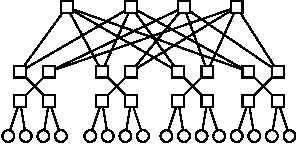
\includegraphics[scale=1.2]{topology-fattree}
        \caption{Fat-tree}%
        \label{fig:topology-fattree}
    \end{subfigure}
    \begin{subfigure}{.45\linewidth}
        \centering
        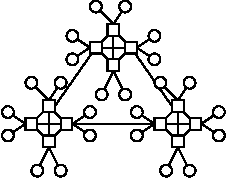
\includegraphics[scale=1.2]{topology-dragonfly}
        \caption{Dragonfly}%
        \label{fig:topology-dragonfly}
    \end{subfigure}
    \par\bigskip
    \begin{subfigure}{.45\linewidth}
        \centering
        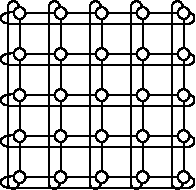
\includegraphics[scale=1.2]{topology-torus}
        \caption{2D Torus}%
        \label{fig:topology-torus}
    \end{subfigure}
    \begin{subfigure}{.45\linewidth}
        \centering
        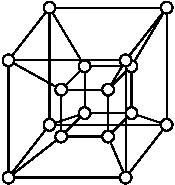
\includegraphics[scale=1.2]{topology-hypercube}
        \caption{4D Hypercube}%
        \label{fig:topology-hypercube}
    \end{subfigure}
    \caption{Topology of Interconnects}%
    \label{fig:topology}
\end{figure}


Mostly, the interconnects of computer cluster systems are full-bisection.
The bisection bandwidth for an interconnect is defined as the minimum
bandwidth between two counterparts of the interconnect. A full-bisection
interconnect is an interconnect whose bisection bandwidth is larger or equal
to the aggregated bandwidth between computing nodes. Interconnects that are
not full-bisection are referred as oversubscribed. Full-bisection interconnect
design are preferred since such interconnect does not suffer from network
contention even in the worst case scenario where all computing nodes
communicate with each other at maximum speed of their network interfaces. This
characteristic is beneficial for application since it removes the need to be
aware of the current contention state of the interconnect. However, there is a
common problem with full-bisection design: the financial cost to implement
such a design increases superlinearly as the number of node scales out.
Therefore, researches are ongoing to effectively utilize oversubscribed
interconnects~\autocite{Leon2017,Michelogiannakis2017} under the assumption
that oversubscribed interconnects become inevitable in the future.

\subsection{Message Passing Interface}\label{sec:i-mpi}

% MPIとは
Message Passing Interface (MPI)~\autocite{MPIForum2012} is a \emph{de
facto} standard specification for inter-process communication libraries
used to develop parallel applications running on distributed memory system
such as clusters. MPI defines a suite of communication primitives that helps
application developers to build parallel distributed applications that require
complex communications among computing nodes.

% 相互結合網の抽象化
A remarkable feature of MPI is that it abstracts the underlying network
of clusters. As shown in Fig.~\ref{fig:mpi-arch}, each interconnect technology
requires the developers to use a different set of APIs. MPI hides the this
incoherence and allows developers to build applications without forcing them
to study the detailed architecture or structure of the underlying network. For
instance, every process is identified by a \emph{rank} number, a consecutive
non-negative integer. The mapping between rank numbers and network addresses
is automatically handled by the MPI library. Communication can be restricted
into a particular group of processes, which is called a \emph{communicator}.
These abstractions make MPI applications portable and easy to be ported to
different computer clusters.

\begin{figure}
    \centering
    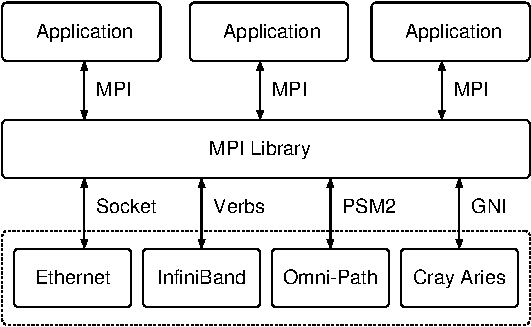
\includegraphics{mpi-arch}
    \caption{Abstraction Provided by MPI}%
    \label{fig:mpi-arch}
\end{figure}

% 1対1通信と集団通信
The communication primitives defined in MPI can be roughly categorized into
point-to-point communication and collective communication. Point-to-point
communication is a communication between one sender and one receiver. On the
other hand, collective communication involves a group of processes. These
communication primitives help application developers to implement complex
parallel algorithms. Table~\ref{tbl:mpi-primitives} shows some representative
examples of MPI primitives.

\begin{table}
    \centering
    \caption{Examples of MPI primitives}%
    \label{tbl:mpi-primitives}
    \begin{tabular}{lll}
        \toprule
        Name & Category & Description \\ \midrule
        MPI\_Send/MPI\_Recv & Point-to-point & Blocking send/receive \\
        MPI\_Isend/MPI\_Irecv & Point-to-point & Non-blocking send/receive \\
        MPI\_Bcast & Collective & Broadcast \\
        MPI\_Reduce & Collective & Reduction \\
        MPI\_Allreduce & Collective & Broadcast result of reduction \\
        MPI\_Gather & Collective & \begin{tabular}[c]{@{}l@{}}Aggregate pieces of data from\\ processes into a single process\end{tabular} \\
        MPI\_Alltoall & Collective & \begin{tabular}[c]{@{}l@{}}Perform MPI\_Gather from all\\ processes\end{tabular} \\
        \midrule
    \end{tabular}
\end{table}

% MPIの高速化
Until today, countless scientific applications have been developed by
utilizing MPI\@. Accompanied by the recent scale-out of clusters, the
execution time of MPI primitives has become a critical factor that determines
the total performance of these applications using MPI\@. In other words, the
total performance of MPI applications can be improved by optimizing the
performance of MPI communications. For this reason, researchers have been
striving to improve the communication performance of MPI from various aspects.

\subsection{Problem and Motivation}

% アプリケーションの通信パターン
The inter-process communication of MPI applications shows a distinctive
pattern. This pattern varies depending on the application and originates from
the mathematical model, discretization method, and parallelization strategy.
Figure~\ref{fig:stencil3d} shows the communication pattern of a
three-dimensional finite-difference solver that performs nearest neighbor
communication as an example. In this figure, the total size of messages sent from
a process to another process is visualized using a heat map. The visual
representation evidently exhibits a regular and local pattern along the
diagonal that originates from the nearest neighbor communication required by
the finite-difference method.
% 論文中の通信パターンの定義をここで書く?

\begin{figure}
    \centering
    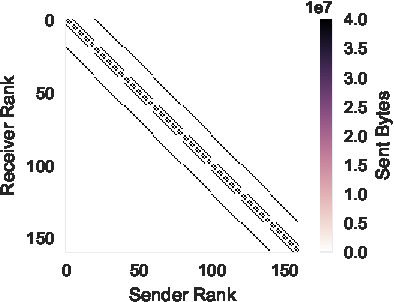
\includegraphics[width=0.6\linewidth]{stencil3d}
    \caption{Communication Pattern of an Application}%
    \label{fig:stencil3d}
\end{figure}

% 相互結合網は通信パターンを無視している
The design of an interconnect could be highly optimized for an
application by taking the communication pattern of applications into account.
For instance, an interconnect with a three-dimensional torus topology would be
ideal for an application that performs nearest neighbor communication in 3D
space. However, this approach is infeasible when designing a real-world
cluster. This is because HPC systems are shared by many users, where each user
runs various applications on the cluster. Furthermore, Therefore, in contrast
to the application-dependent communication pattern, the interconnect is
inherently application-agnostic.

% 問題
As a result, under a certain combination of communication pattern and
interconnect, an imbalance of the packet flow in the interconnect can occur.
The imbalance can lead to the concentration of traffic on a link in the
interconnect and slow down of MPI communication that uses the link. The
degraded MPI communication can ultimately lead to a serious degradation of
total application performance.

% 関連研究
A  number of previous studies have tried to address the mismatch between
application application-dependent communication patterns and
application-agnostic interconnects. A class of approaches tries to adapt
the communication pattern of applications to the interconnect.
For instance, interconnect-aware MPI
collectives~\autocite{Kumar2016,Kumar2014,Gong2015,Adachi2013} have been
developed to improve the performance of MPI collectives by taking into account
the interconnect of a cluster. MPI implementation often leverage tree-based
algorithms to aggregate or distribute messages from or to processes.
Interconnect-aware MPI collectives use the information on the interconnect to
build a delivery tree that matches the underlying interconnect of the cluster.
Another class of approaches tries to optimize the placement of MPI processes
on the computing nodes~\autocite{Michelogiannakis2017,Hoefler2011,Choi2017}.
In this approach, the communication pattern of an application is considered as
a weighted graph where nodes represent processes and edges represent the
volume of data exchanges between two processes. Various heuristic algorithms
are proposed to embed the communication pattern graph graph onto the
interconnect topology.

% 相互結合網の動的制御は未だ研究が進んでいない
To this date, however, there has been little studies on adapting the
interconnect to the communication pattern of applications. This is mostly
because it has been assumed that flexibly and dynamically reconfiguring the
interconnect at runtime is infeasible. However, this assumption might not hold
anymore with the recent emergence of programmable networking architecture that
allows reconfiguring the interconnect on-the-fly.

\subsection{Software-Defined Networking}

% SDN
Software-Defined Networking (SDN) is a novel networking architecture
that separates the control plane and data plane into different devices.
In conventional networking architectures, the decision on how to handle
packets (control plane) and the packet transfer (data plane) are
implemented as unified and inseparable features. The separation of the
control plane and data plane has allowed SDN to deliver the following
three benefits:

\begin{itemize}
\item
  \emph{Programmable}: The control plane can be handled by a software
  controller. Network operators can program controllers tailored for
  their needs.
\item
  \emph{Dynamic}: SDN allows the controller to quickly reconfigure the
  network. For instance, it is possible to dynamically optimize packet
  flow in the network based on the real-time traffic pattern.
\item
  \emph{Centralized}: A centralized controller configures the entire
  SDN-enabled network, thus reducing efforts to administer and manage
  the network. In conventional networking architectures, the operators
  need to configure each network device separately because the control
  plane is distributed on individual devices.
\end{itemize}

\begin{figure}
    \centering
    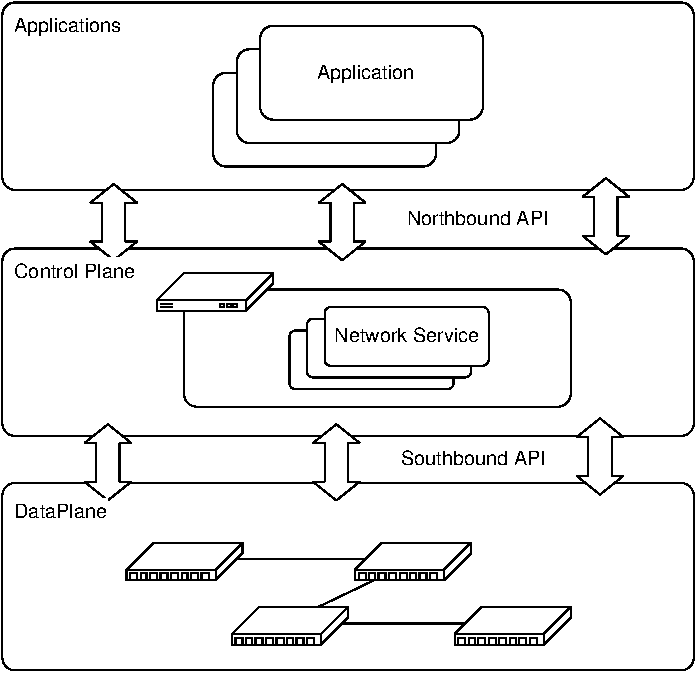
\includegraphics{sdn}
    \caption{Software-Defined Networking Architecture}%
    \label{fig:sdn-architecture}
\end{figure}

% OpenFlow
\emph{OpenFlow}~\autocite{McKeown2008} is a widely accepted open
standard of SDN\@. In an OpenFlow-enabled network, the data plane is
handled by OpenFlow switches. Every OpenFlow switch holds a logical
construct called \emph{flow table}, which is a collection of \emph{flow
entries}. Each flow entry defines what kind of packet control should be
performed on what kind of packets (Fig.~\ref{tbl:flow-table}). Every
time a packet arrives at an OpenFlow switch, the switch looks up a
matching flow entry in its flow table using the header fields of the
packet. Once a matching flow entry is found, the action of the matched
flow entry is applied to the packet.

The OpenFlow controller is responsible for the control plane. It manages
the flow table of switches by adding, removing and modifying flow
entries. The controller and switches communicate with each other by
asynchronously exchanging messages defined in the OpenFlow protocol. One
of the frequently used messages is the \emph{packet-in} message, which
is sent out from a switch to the controller when no matching flow entry
is found for an incoming packet. In response, the controller can send a
\emph{modify flow entry} message to install a new flow entry on the
switch.

\begin{figure}
    \centering
    \begin{tabular}{lllll}
        \toprule
        \multicolumn{3}{c}{Header Fields}            &  Action                  \\ \midrule
        Dst MAC           & Src IP     & Dst IP      &                          \\ \midrule
                          & 192.0.2.12 & 192.0.2.34  & Output to port 1         \\
                          & 192.0.2.34 & 192.0.2.56  & Output to port 2         \\
        ff:ff:ff:ff:ff:ff &            &             & Output to port 1 and 2   \\
        72:42:c1:e4:75:8c &            &             & Drop                     \\
        \bottomrule
    \end{tabular}
    \caption{An example of a flow table}%
    \label{tbl:flow-table}
\end{figure}

% もう一枚図を追加?

\section{Research Objective}

As discussed in Section~\ref{sec:i-background}, the mismatch between
application-dependent communication patterns and application-agnostic
interconnects have lead to the imbalance of packet flow in the interconnect.
This dissertation aims to address this problem by establishing a programmable
interconnect control that dynamically controls the packet flow in the
interconnect based on the communication pattern of applications.

\begin{figure}
    \centering
    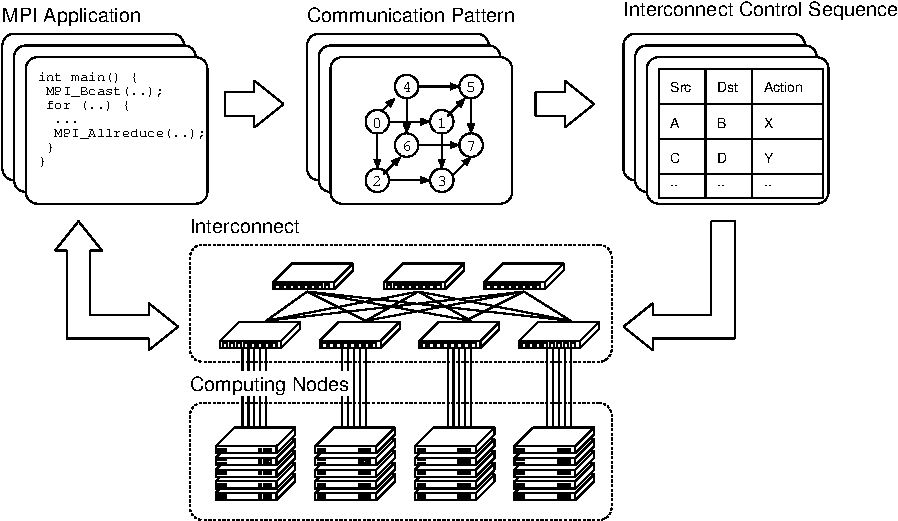
\includegraphics{objective}
    \caption{Envisioned Interconnect Control}%
    \label{fig:objective}
\end{figure}

Figure~\ref{fig:objective} illustrates the envisioned interconnect control
architecture. The overall idea of this architecture is as follows. First, the
communication pattern of MPI communication is extracted from the application.
Then, a sequence of interconnect control instructions is generated based on
the communication pattern. Finally, the interconnect control sequence is
applied to the interconnect using programmable interconnect technology.
There are three central challenges in realizing such programmable interconnect:

\begin{enumerate}
\item \emph{Analyzing the Packet Flow in the Interconnect}:
    To effectively control the packet flow in the interconnect, we first need
    to analyze and understand the packet flow generated in the interconnect
    when running an application on the cluster.
\item \emph{Accelerating MPI Communication by Dynamic Control of Interconnect}:
    Given a communication pattern of an application and an interconnect,
    we need to determine how to control the packet flow in the interconnect to
    mitigate imbalance and improve the performance of MPI communication.
\item \emph{Coordinating the Execution of Application and Interconnect Control}:
    The communication pattern of the application changes with the execution of
    the application. Therefore, the interconnect control must be performed in
    accordance with the execution of application.
\end{enumerate}

\section{Organization of the Dissertation}

The rest of this dissertation is organized as follows:

% アプリケーションが相互結合網内に生成するパケット
フローの解析手段を実現
In Chapter~\ref{sec:ii}, we propose PFAnalyzer, a toolset for analyzing packet
flow in interconnects to address the first challenge. Interconnect simulators
come in handy especially when investigating the performance characteristics of
interconnects with different topologies and parameters. However, little effort
has been put towards the simulation of packet flow in dynamically controlled
interconnects, while simulators for static interconnects have been extensively
researched and developed. To facilitate analysis on the performance
characteristics of dynamic interconnects, we have developed PFAnalyzer.
PFAnalyzer is a pair of two tools: PFSim, an interconnect simulator
specialized for dynamic interconnects, and PFProf, a profiler. PFSim allows
interconnect researchers and designers to investigate congestion in the
interconnect for an arbitrary cluster configuration and a set of communication
patterns collected by PFProf. PFAnalyzer is used to demonstrate how
dynamically controlling the interconnects can reduce congestion and
potentially improve the performance of applications.

% MPI集団通信を高速化するパケットフロー制御アルゴリズムを配備可能なフレームワークを構築
In Chapter~\ref{sec:iii}, we address the second challenge by proposing a
framework that accelerates MPI collectives by controlling the packet flow in
the interconnect. We integrate the network programmability provided by
Software-Defined Networking into MPI collectives so that collectives are able
to effectively utilize the bandwidth of the interconnect. In particular, we
aim to reduce the execution time of MPI\_Allreduce, a frequently used MPI
collective communication in many simulation codes. An experiment conducted on
a cluster system with fat-tree interconnect indicates that our proposed
MPI\_Allreduce is superior to MPI\_Allreduce in Open MPI implementations.

% 通信と計算が連係動作する新たなクラスタアーキテクチャを確立
In Chapter~\ref{sec:iv}, the third challenge is addressed. This chapter
proposes UnisonFlow, a software-defined coordination mechanism that performs
network control in synchronization with the execution of applications. An
experiment conducted on a real computer cluster verifies that the interconnect
control can be successfully performed in synchronization with the execution of
the application. Furthermore, the synchronization is performed with a low
overhead and its performance penalty is practically negligible.

Chapter~\ref{sec:v} concludes this dissertation and describes the future work.

\chapter{Toolset for Analyzing Packet Flow in Interconnect}\label{sec:ii}

\section{Introduction}\label{sec:ii-introduction}

Inter-node communication performance of high-performance computing~(HPC)
clusters heavily affects the total performance of
communication-intensive applications. Communication-intensive
applications require low-latency and high-bandwidth communication
between compute nodes to fully exploit the computational power and
parallelism of the compute nodes. High performance networks that
provide such low-latency and high-bandwidth communication between
compute nodes of a cluster are often referred to as
\emph{interconnects}. Message Passing Interface
(MPI)~\autocite{MessagePassingInterfaceForum2015,Gropp2014} is a
commonly used inter-process communication library to describe
communication on HPC clusters.

In this dissertation, the interconnects are roughly classified into
\emph{static interconnects} and \emph{dynamic interconnects}. In the former
category, it is assumed that packet flow is statically controlled solely based
on its source and/or destination. A well-known exemplifier is
InfiniBand~\autocite{Buyya2009}, where forwarding tables held by switches are
populated with pre-computed forwarding rules in advance of the execution of
applications. In contrast, in the latter category, it is assumed that packet
flow is dynamically controlled to mitigate load imbalance and improve
utilization of the interconnect.

Nowadays, the majority of HPC clusters employ the former static interconnects
because of their technological maturity despite the potential cost advantage
dynamic interconnects could provide. The static interconnects are controlled
without taking the communication patterns of individual applications into
account. However, they are usually designed to be able to accommodate the
worst-case traffic demand to achieve good performance for a variety of
applications, each of which has a different communication pattern.
Interconnect designers have respected such criteria as full bisection
bandwidth and non-blocking networks.

The continuously growing demand for computing power from academia and
industry has inevitably forced HPC clusters to scale out more and more.
As a result of the growing number of compute nodes, interconnects
have been increasingly large-scale and complex. This technical trend is making
static and over-provisioned interconnects more cost-ineffective and
difficult to build.

Based on this background and these trends, this study explores the feasibility
and applicability of programming dynamic interconnect within
HPC~\autocite{Date2016}. In particular, \emph{SDN-enhanced
MPI}~\autocite{Takahashi2014,Dashdavaa2013}, a framework that incorporates
the dynamic network controllability of Software-Defined Networking
(SDN)~\autocite{sdn} into MPI, has been researched based on the idea that
dynamically optimizing the packet flow in the interconnect according to the
communication patterns of applications can increase the utilization of the
interconnect and then improve application performance. The goal of
SDN-enhanced MPI is to accelerate individual MPI collectives by dynamically
optimizing the packet flow in the interconnect. Several MPI collectives have
been successfully accelerated in the previous works up to this time. One of
the core challenges in the research on SDN-enhanced MPI lies in the design of
an algorithm to effectively control the packet flow in the interconnect for
each MPI collective called by the application.

More generally, an algorithm that takes the communication patterns of
applications as its input and then determines how to manage the packet flow
is essential towards realizing a dynamic and application-aware interconnect.
In order to develop a generic algorithm that achieves good performance on a
variety of applications and interconnects, the algorithm must be investigated
and evaluated by targeting different applications and interconnects. However,
utilizing actual clusters to analyze the performance characteristics of the
interconnect is restricted in the following three points. First, the execution
time of real-world HPC applications typically ranges from hours up to days,
sometimes even months. Second, large-scale deployments of dynamic
interconnects that allow execution of highly parallel applications have not
yet been seen because the research and development of dynamic interconnects
are still at their early stage. Third, network hardware such as switches may
not support measuring traffic in the interconnect with enough high frequency
and precision to obtain meaningful insights.

From the three restrictions mentioned above, an interconnect simulator that
allows researchers to conduct a systematic investigation of clusters with
diverse topologies and parameters is essentially demanded to accelerate the
research and development of application-aware dynamic interconnects that
control packet flow in response to the communication patterns of applications.
A wide spectrum of interconnect simulators have been developed with different
focus and purpose until today. However, existing simulators mostly focused on
static interconnects and few research has been done to simulate dynamic and
application-aware interconnects.

This chapter describes the design and implementation of PFAnalyzer, a
toolset for analyzing application-aware dynamic interconnects.
PFAnalyzer consists of two components: PFSim and PFProf. PFSim is an
interconnect simulator specialized for application-aware dynamic
interconnects. PFSim takes a set of communication patterns derived from
applications and a cluster configuration as its input and then simulates the
traffic on each link of the interconnect. PFProf is a custom profiler to
extract communication patterns from applications which are supplied to PFSim.

The contributions of this chapter are summarized as follows:

\begin{itemize}
\item
  A lightweight interconnect simulator for simulating dynamic and
  application-aware interconnects is proposed.
\item
  A custom profiler for extracting communication patterns from
  applications is presented.
\item
  Simulation results for NAS CG benchmark and MILC on a fat-tree
  interconnect are presented to demonstrate the practicality of of the
  proposed toolset.
\end{itemize}

The rest of this chapter is organized as follows.
Section~\ref{sec:ii-objective} examines the requirements of an
interconnect simulator for dynamic and application-aware interconnects.
Section~\ref{sec:ii-proposal} describes the design and implementation of
PFAnalyzer. Section~\ref{sec:ii-evaluation} evaluates the accuracy of the
simulated traffic. Furthermore, the NAS CG benchmark and MILC are taken as
example applications to demonstrate how PFAnalyzer can be used by researchers
to analyze the joint effect of node allocation, process placement and routing
on the distribution of traffic in the interconnect.
Section~\ref{sec:ii-related-work} reviews the related work.
Section~\ref{sec:ii-conclusion} concludes this chapter and outlines future
work.

\section{Research Objective}\label{sec:ii-objective}

% 大目標・シミュレーションを採用する理由
This chapter aims to realize a toolset for analyzing the packet flow in the
interconnect to facilitate the research and development of application-aware
dynamic interconnects. The packet flow generated in an interconnect highly
depends on parameters such as the communication pattern of application,
interconnect design and cluster configuration. When designing and implementing
an efficient application-aware dynamic interconnect, researchers need to
conduct a systematic analysis over many combinations of these parameters.
However, conducting such analysis on a physical cluster can be extremely time-
and resource-consuming. Therefore, this research takes the approach of
utilizing simulation to facilitate the analysis.

This research attempts to provide a toolset that performs a lightweight
simulation of the interconnect and predicts the packet flow generated in the
interconnect. The toolset should allow researchers to predict the packet flow
in the interconnect by supplying the communication pattern of real-world
application alongside with the interconnect design and cluster configuration.
The predicted packet flow can then be analyzed by researchers to gain an
insight on the interconnect while significantly saving the time and cost
compared to experiments on a physical cluster. Based on the discussion above,
the toolset should be able to satisfy the following requirements.

\begin{itemize}
\item
  \emph{Extraction of communication patterns from applications}:
  Communication patterns of real-world HPC applications should be fed
  into the simulator to reproduce the characteristics of communication
  generated by real-world applications. To simulate the packet flow in
  the interconnect when an application is being executed, the simulator
  needs to predict the volume of point-to-point communication exchanged
  between compute nodes. In the actual computing scene, the traffic
  among compute nodes is generated by the processes executed on the
  compute nodes. Thus, some means to analyze the traffic volume of
  point-to-point communication exchanged between the processes from
  applications is essential. In this chapter, applications that leverage
  MPI for inter-process communication are targeted.
\item
  \emph{Reproduction of process placement characteristic}:
  As described in Section~\ref{i:cluster-arch}, multiple jobs are running
  concurrently on a real-world cluster. Under such a cluster environment, the
  process placement characteristic of the job scheduler such as job
  scheduling, node selection and process placement algorithms heavily affect
  the distribution of packet flow generated in the interconnect. Since the
  job scheduler and its configuration largely varies across deployments,
  the process placement characteristic of the job scheduler needs to be
  reproduced.
\item
  \emph{Efficient prediction of packet flow in the interconnect}:
  The simulator should be designed to be lightweight and fast
  to carry out a large number of simulations with different parameters in
  a reasonable amount of time. If necessary, appropriate approximation
  should be introduced to improve simulation performance.
\end{itemize}

\section{Proposal}\label{sec:ii-proposal}

This research proposes \emph{PFAnalyzer}, a toolset for analyzing the
performance characteristics of application-aware dynamic interconnects.
PFAnalyzer is composed of \emph{PFProf}, a profiler to extract communication
patterns from applications, and \emph{PFSim}, a simulator capable of
simulating application-aware dynamic interconnects.

\subsection{Representation of a Communication Pattern}

In this dissertation, the communication pattern of an application is
represented using a traffic matrix of the application. The reason why this
research has adopt traffic matrix as representation of communication pattern
is explained below.

The traffic matrix of an application is defined as a matrix of which element
is equal to the traffic volume exchanged between two processes in the
application. Here, the volume of traffic between processes is approximated as
being constant during the execution of a job. In other words, the traffic
volume between a process pair is assumed to be the total bytes transferred
divided by the runtime of the application.

This approximation is introduced to reduce the size of the communication
pattern as well as to simplify and to speed up the simulation. The idea behind
this approximation is based on the fact that many HPC applications
(\emph{e.g.} partial differential equation solvers) exhibit an iterative
nature. These applications spend most of their execution time inside a
repetitive loop and thus their communication patterns do not significantly
change over time. Therefore, omitting the temporal change of the communication
pattern and assuming the traffic volume between processes as being constant is
a good approximation. In the future, trace segmentation~\autocite{Alawneh2016}
techniques can be applied on the communication trace. This technique
segments a trace into multiple communication phases, which could then be
simulated individually to further improve the accuracy of simulation for
applications with significantly time-varying communication patterns.

\subsection{PFProf (MPI Profiler)}\label{sec:ii-pfprof}

% PFProfの概要
PFProf is a profiler that extracts the inter-process communication patterns
from MPI applications. The collected communication patterns are later fed into
PFSim to simulate the packet flow generated in the interconnect.

% プロファイリングを使う理由
To capture the inter-process communication of an MPI application, either
profiling or static analysis is commonly utilized. Profiling gives accurate
results but requires the users to run their application once. In contrast,
static analysis of the source code does not require the users to run their
application. However, the communication patterns obtained through the use of
static analysis are usually less accurate compared to the patterns obtained by
profiling. This research takes the profiling approach because an accurate
communication pattern is essential to obtain a simulation result with high
fidelity.

% PMPIの問題点
Initially, existing MPI profilers and tracers such as
\mbox{Score-P}~\autocite{Knupfer2012}, Vampir~\autocite{Knupfer2008} and
TAU~\autocite{Shende2006} were considered for collecting the traffic matrices
from MPI applications. However, these tools can capture only a subset of the
communication pattern when profiling an application that uses MPI collectives.
The reason can be explained from the following technological aspect. Existing
MPI profilers replace the standard MPI functions provided by MPI libraries
with instrumented functions by utilizing the MPI Profiling Interface~(PMPI).
Although this approach works regardless of a specific MPI implementation, it
fails to capture the function calls made within the MPI library. Meanwhile,
collective communication functions are internally implemented as a combination
of point-to-point communication in MPI implementations. These underlying
point-to-point communication functions are hidden from PMPI-based profilers
and excluded from the communication patterns emitted by profilers.

% 集団通信を実現するアルゴリズムによっても変わる
Furthermore, the combination of point-to-point communication that composes a
collective communication is unknown until the collective communication
function is called during the execution of the application. This is because
MPI libraries usually implement multiple algorithms for each MPI collective
that are selected depending on the message size and number of processes. For
example, Open~MPI~\cite{Gabriel2004} implements three algorithms to realize
MPI\_Allgather: the recursive doubling algorithm, the Bruck algorithm, and the
ring algorithm~\cite{Rabenseifner2004}. Figure~\ref{fig:allgather-algorithms}
illustrates the underlying point-to-point communication of MPI\_Allgather for
each algorithm. It is evident that the point-to-point communication of
MPI\_Allgather is significantly different depending on the algorithm being
used.

\begin{figure}
    \centering
    \begin{subfigure}{\linewidth}
        \centering
        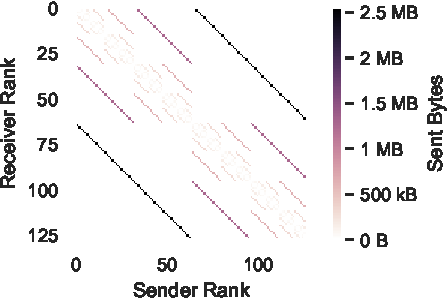
\includegraphics[width=.57\linewidth]{allgather_recursive_doubling}
        \caption{Recursive Doubling Algorithm}%
        \label{fig:allgather-recursive}
    \end{subfigure}
    \begin{subfigure}{\linewidth}
        \centering
        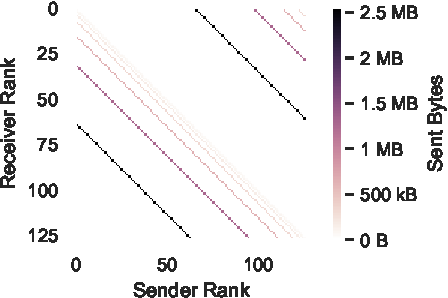
\includegraphics[width=.57\linewidth]{allgather_bruck}
        \caption{Bruck Algorithm}%
        \label{fig:allgather-bruck}
    \end{subfigure}
    \begin{subfigure}{\linewidth}
        \centering
        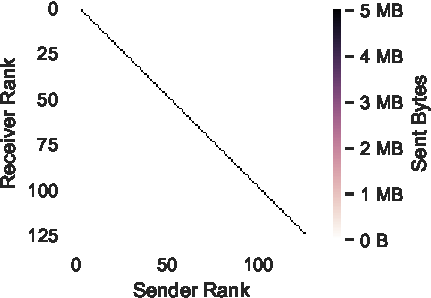
\includegraphics[width=.57\linewidth]{allgather_ring}
        \caption{Ring Algorithm}%
        \label{fig:allgather-ring}
    \end{subfigure}
    \caption{Underlying Point-to-Point Communication of MPI\_Allgather}%
    \label{fig:allgather-algorithms}
\end{figure}

% PERUSEを採用する理由
To accurately capture the underlying point-to-point communication of
collective communication, this research has taken the strategy of utilizing
the MPI Performance Examination and Revealing Unexposed State Extension
(PERUSE)~\autocite{Jones2006}. PERUSE was designed to provide the internal
information of an MPI implementation that was not exposed through PMPI to
applications and performance analysis tools. PERUSE delivers the internal
information of an MPI implementation to applications and performance analysis
tools through an event-driven API\@.

% アプリケーションの実行前の動作
Figure~\ref{fig:profiler-block} illustrates how PFProf, the MPI library and an
MPI application interact with one another. PFProf intercepts the function
calls from the application to several MPI functions using PMPI\@. MPI\_Init
and MPI\_Finalize are intercepted to perform initialization and finalization
when the application starts or exits (step~1 in
Fig.~\ref{fig:profiler-block}). In addition, PFProf intercepts MPI functions
that create or destroy communicators to maintain a mapping between global
ranks (rank number within \lstinline!MPI_COMM_WORLD!) and local ranks (rank
number within a communicator created by the user). This mapping is necessary
because PERUSE events are reported with local ranks, while profiling results
should be described with global ranks for the ease of analysis. During the
initialization, PFProf subscribes to two PERUSE events:
\lstinline!PERUSE_COMM_REQ_XFER_BEGIN! and
\lstinline!PERUSE_COMM_REQ_XFER_END! (step~2). These events are emitted each
time a transfer of a message begins and ends, respectively.

\begin{figure}
    \centering
    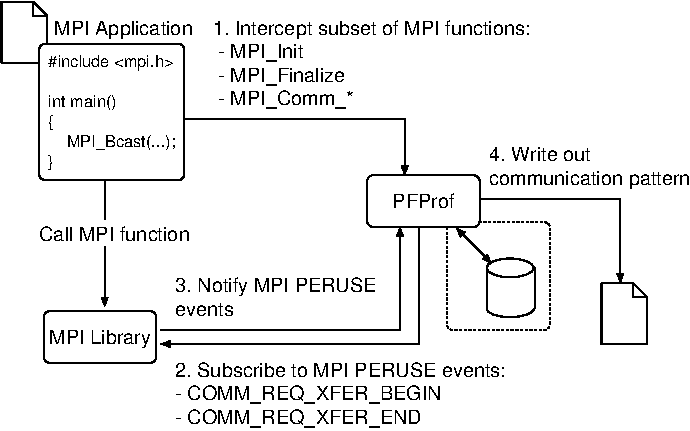
\includegraphics{tracer_block}
    \caption{Block Diagram of PFProf}%
    \label{fig:profiler-block}
\end{figure}

% アプリケーションの実行開始後の動作
After the application starts, PFProf receives PERUSE events from the MPI
library every time the application calls an MPI function that causes
inter-process communication (step~3). PERUSE extracts the sender, receiver and
transferred bytes from each PERUSE event and updates the traffic matrix
online. Once the application calls MPI\_Finalize, the communication pattern is
written out to disk as a JSON file (step~4).

% 共有ライブラリ
Finally, PFProf is designed to be provided in the form of a shared library so
that users do not need to modify the source code of their applications. Users
can either set the \lstinline!LD_PRELOAD! environment variable to load the
shared library at run-time or dynamically link the shared library with their
application at build-time.

\subsection{PFSim (Interconnect Simulator)}\label{sec:ii-pfsim}

% PFSimの概要
PFSim uses a set of communication patterns of applications and a cluster
configuration as its input and then simulates the packet flow generated
by the applications. The packet flow is aggregated per link to compute
the traffic load on each link. The simulated traffic load of links can
be summarized into statistics for quantitative analysis or visualized.
Using these outputs from PFSim, users can locate hot-spots and assess
load imbalance in the interconnect. These insights on the interconnect
can be useful for designing better algorithms for controlling the packet
flows in application-aware dynamic interconnects.

% シミュレーションの方式とモデル
Methodologies for simulating interconnects are roughly classified into
packet-level simulation~\cite{Hoefler2010} and flow-level
simulation~\cite{Schneider2009}. In the packet-level simulation, the behavior
of how each packet travels through the interconnect is precisely reproduced.
Therefore, the communication time of applications can be predicted accurately
in exchange for long execution time and large memory foot print. In contrast,
the flow-level simulation estimates the steady state behavior of the
interconnect and does not track individual packets. Thus, the packet flow in
the interconnect can be speedily estimated compared to the packet-level
simulation. As a trade-off, predicting the communication time of applications
using flow-level simulation is challenging. As described in
Section~\ref{sec:ii-objective}, this research aims at realizing a toolset for
efficiently predicting the packet flow in the interconnect under diverse
configurations. Therefore, PFSim is based on the flow-level simulation for
execution efficiency.

% シミュレータの構造
Figure~\ref{fig:pfsim-arch} shows the internal structure of PFSim. This
simulator is based on a discrete-event simulation model. Under this model, the
simulation is driven by events, each of which indicates a change in the
internal state of the simulator. Each event holds (1) type of the event, (2)
time when the event will occur, and (3) additional information indicating what
kind of state change the event will cause. An event queue is a priority queue
that stores the events prioritized by the time each event occurs. An event
handler is a function that is associated to a specific event type and invoked
when an event of the associated type occurs. The dispatcher manages the event
queue. It pops events from the event queue one by one and calls the associated
event handler for each event.

\begin{figure}
    \centering
    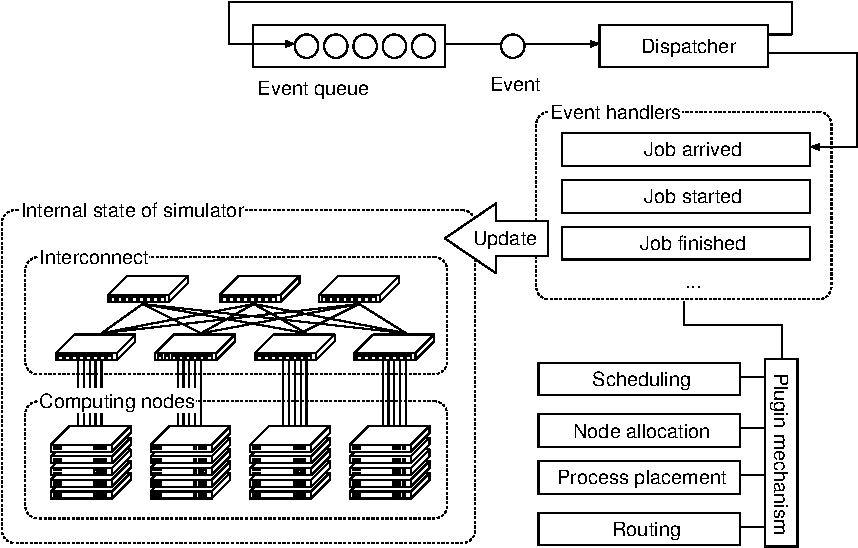
\includegraphics{pfsim-arch}
    \caption{Internal Structure of PFSim}%
    \label{fig:pfsim-arch}
\end{figure}

% ジョブ到着イベントハンドラ
In PFSim, three event types exist: job-arrived, job-started and job-finished.
The event handler for the job-arrived event first checks if the job queue is
empty and if there are enough compute nodes unallocated to run the job. If the
job is not runnable at the time, the job is enqueued to the job queue and the
event handler finishes. If the job is runnable, the event handler initiates
the job startup routine shown in Algorithm~\ref{alg:start-job}. First, a set
of available compute nodes are allocated to the job (line 1 in
Algorithm~\ref{alg:start-job}). Next, the placement of processes on the
allocated compute nodes is determined (line 2--3). Subsequently, each process
is associated to the compute node that accommodates it (line 4--5). Finally, a
job-started event is inserted into the event queue (line 6).

\begin{algorithm}
    \SetKwData{Job}{job}
    \SetKwData{Node}{node}
    \SetKwData{Nodes}{nodes}
    \SetKwData{Proc}{proc}
    \SetKwData{Procs}{procs}
    \SetKwData{Mapping}{mapping}
    \SetKwFunction{allocateNodes}{allocateNodes}
    \SetKwFunction{testNodes}{testNodes}
    \SetKwFunction{mapProcs}{mapProcs}

    \Nodes $\gets$ \allocateNodes{\Job}\;
    \Procs $\gets$ Set of processes composing \Job\;
    \Mapping $\gets$ \mapProcs{\Procs, \Nodes}\;
    \ForEach{(\Proc, \Node) $\in$ \Mapping}{%
        Associate \Proc with \Node\;
    }
    Insert job-started event to event queue\;

    \caption{Job start routine}%
    \label{alg:start-job}
\end{algorithm}

% ジョブ開始イベントハンドラ
Algorithm~\ref{alg:on-job-started} shows the overview of the event handler for
the job-started event. This event handler first obtains the traffic matrix of
the application that has started (line 1 in
Algorithm~\ref{alg:on-job-started}). Next, based on the traffic matrix, the
traffic load on each link in the interconnect is updated as follows: first,
compute nodes that accommodate the source and destination processes are
obtained (line 3--4). Subsequently, the path from the source compute node to
destination compute node is calculated (line 5--8). Lastly, the traffic load
on each link along the path is increased based on the amount of traffic
transferred between the source and destination processes (line 9--10). After
the traffic load is updated, the event handler inserts a job-finished event
into the job queue (line 11).

\begin{algorithm}
    \SetKwData{Job}{job}
    \SetKwData{SrcProc}{srcProc}
    \SetKwData{DstProc}{dstProc}
    \SetKwData{SrcNode}{src}
    \SetKwData{DstNode}{dst}
    \SetKwData{Link}{link}
    \SetKwData{Path}{path}
    \SetKwData{Traffic}{traffic}
    \SetKwData{TrafficMatrix}{tm}
    \SetKwFunction{route}{route}
    \SetKwFunction{selectJob}{selectJob}

    \TrafficMatrix $\gets$ Traffic matrix of \Job\;
    \ForEach{(\SrcProc, \DstProc, \Traffic) $\in$ \TrafficMatrix}{%
        \SrcNode $\gets$ Compute node that accommodates \SrcProc\;
        \DstNode $\gets$ Compute node that accommodates \DstProc\;
        \If{path between (\SrcNode, \DstNode) is already computed}{%
            \Path $\gets$ Cached path between (\SrcNode, \DstNode)\;
        }
        \Else{%
            \Path $\gets$ \route{\SrcNode, \DstNode, \Job}\;
        }
        \ForEach{\Link $\in$ \Path}{%
            Increase traffic load of \Link for \Traffic\;
        }
    }
    Insert job-finished event to event queue\;

    \caption{Event Handler for Job-started Event}%
    \label{alg:on-job-started}
\end{algorithm}

% ジョブ終了イベントハンドラ
The event handler for the job-finished event releases the compute nodes
allocated to the job. If there are one or more jobs in the job queue, one of
them is selected. If there are enough number of available compute nodes, the
job startup routine shown in Algorithm~\ref{alg:start-job} is invoked.

% シミュレーションシナリオファイルの概要
PFSim aims at predicting the packet flow in the interconnect generated by
applications under diverse cluster configurations. The configuration of the
simulation must be able to be edited by users. For the reason, the
configuration is described in a human-readable \emph{simulation scenario}
file. The simulation scenario file is designed to be described in a structured
serialization format called YAML\@. YAML has been adopted for its high
readability and editability compared to other alternatives such as JSON and
XML\@.

% シミュレーションシナリオファイルの詳細
Listing~\ref{lst:simulation-scenario} shows an example of a simulation
scenario file. In this simulation scenario file, the topology of the
interconnect (line 1 in Listing~\ref{lst:simulation-scenario}), output
directory for the simulation results (line 2), and a set of jobs to simulate
(line 16--21) are specified. Moreover, the algorithms that control the
execution and communication of jobs, which are shown in
Table~\ref{tbl:simulator-algorithm}, are also specified (line 3--15). Each
configuration value can be a list of parameters. The simulation is executed
multiple times, each time with a different combination of configuration values
until all combinations are completed. In
Listing~\ref{lst:simulation-scenario}, one scheduling algorithm (line 4--5),
two node allocation algorithms (line 6--8), two process placement algorithms
(line 9--11), and three routing algorithms (line 12--15) are specified. When
this scenario file is supplied to PFSim, 12 simulations are executed in total
in a combination manner.

\begin{lstlisting}[caption={Example of a Simulation Scenario},%
                   label={lst:simulation-scenario}, linewidth={\columnwidth},%
                   float={htbp}]
topology: topologies/milk.graphml
output: output/milk-cg-dmodk
algorithms:
  scheduler:
    - pfsim.scheduler.FCFSScheduler
  node_selector:
    - pfsim.node_selector.LinearNodeSelector
    - pfsim.node_selector.RandomNodeSelector
  process_mapper:
    - pfsim.process_mapper.LinearProcessMapper
    - pfsim.process_mapper.CyclicProcessMapper
  router:
    - pfsim.router.DmodKRouter
    - pfsim.router.GreedyRouter
    - pfsim.router.GreedyRouter2
jobs:
  - submit:
      distribution: pfsim.math.ExponentialDistribution
      params:
        lambd: 0.1
    trace: traces/cg-c-128.tar.gz
\end{lstlisting}

\begin{table}
    \centering
    \normalsize
    \caption{List of Configurable Algorithms}%
    \label{tbl:simulator-algorithm}
    \begin{tabularx}{\linewidth}{lX}
        \toprule
        Algorithm         & Description                                                 \\
        \midrule
        Job Scheduling    & Selects the job to execute from the job queue.
                            (\emph{e.g.} FCFS, Backfill)                                \\
        Node Selection    & Selects which compute nodes to assign for a job.
                            (\emph{e.g.} Linear, Random, Topology-aware algorithms)     \\
        Process Placement & Determines on which compute node to place a process.
                            (\emph{e.g.} Block, Cyclic, Application-aware algorithms)   \\
        Routing           & Computes a route between a pair of processes.
                            (\emph{e.g.} D-mod-K, S-mod-K, Random, Dynamic algorithms)  \\
        \bottomrule
    \end{tabularx}
\end{table}

Since PFSim accepts the topology of the interconnect as its input and outputs
the traffic load on each link of the interconnect, the file format for
representing the interconnect needs to be considered. The file format should
be designed for graphs since the interconnect can be considered as a graph. In
addition, the format should be supported by existing analysis and
visualization tools so that users can take advantage of these software assets.
Based on the requirements above, PFSim is designed to use
GraphML~\autocite{Brandes2013}, an XML-based markup language for graphs, as
its input and output format of the interconnect. Popular graph visualization
tools such as Cytoscape and Gephi can be used to view and edit GraphML files.
Users can use these tools to visually and intuitively locate bottleneck links
and load imbalance in the simulated interconnect.

\section{Evaluation}\label{sec:ii-evaluation}

The first experiment is conducted to verify if PFProf is able to capture
the underlying point-to-point communication behind collective communication.
Then, the accuracy of the simulation performed by PFSim is evaluated through
the comparison of the traffic estimated by PFSim with the traffic measured on
a cluster when actually running an application. Then, the performance of
point-to-point communication between two processes with and without PFProf are
compared to assess the overhead incurred by PFProf. Lastly, how PFAnalyzer can
be used by researchers to analyze the joint effect of node allocation, process
placement and routing on the distribution of traffic in the interconnect is
demonstrated.

\subsection{Comparison of PFProf and Conventional Profiler}%
\label{sec:ii-eval-pfprof}

This experiment verifies if PFProf is able to capture the underlying
point-to-point communication of collective communication. A simple
MPI application is profiled using TAU and PFProf. Subsequently, the extracted
communication patterns are compared. Listing~\ref{lst:pfprof-example} shows
the source code of the MPI application. This application first executes
MPI\_Allreduce, one of the commonly used collective communications. Then,
every process performs a point-to-point communication with its neighboring
process. This application is executed with 128 processes.

Figure~\ref{fig:tau-comm-matrix} shows the communication pattern obtained with
TAU\@. In this figure, the horizontal and vertical axis indicate the sender and
receiver rank, respectively. The point-to-point communication between the
neighbor processes is clearly visualized as a pattern along the diagonal.
However, the underlying point-to-point communication of MPI\_Allreduce was not
observed. On the other hand, Figure~\ref{fig:pfprof-comm-matrix} shows the
communication pattern obtained with PFProf. This communication pattern reveals
the MPI communication generated from MPI\_Allreduce in detail. The underlying
point-to-point communication is clearly detailed. These observations suggest
that PFProf is able to capture the underlying point-to-point communication of
collective communication.

\begin{lstlisting}[caption={MPI Application Used for Evaluation},
                   label=lst:pfprof-example, float, language=C]
#include <stdio.h>
#include <mpi.h>

#define BUF_SIZE    (1000)

int rank, size;
MPI_Request req;
char buf[BUF_SIZE] = {};
char buf2[BUF_SIZE] = {};

int main(int argc, char *argv[])
{
    MPI_Init(&argc, &argv);

    MPI_Comm_rank(MPI_COMM_WORLD, &rank);
    MPI_Comm_size(MPI_COMM_WORLD, &size);

    /* Collective communication */
    MPI_Allreduce(buf, buf2, BUF_SIZE, MPI_CHAR,
                  MPI_SUM, MPI_COMM_WORLD);
        \label{fig:allgather-ring}

    /* Point-to-point communication */
    MPI_Irecv(buf, BUF_SIZE, MPI_CHAR,
              (rank - 1) % size,
              0, MPI_COMM_WORLD, &req);
    MPI_Send(buf, BUF_SIZE, MPI_CHAR,
             (rank + 1) % size,
             0, MPI_COMM_WORLD);
    MPI_Wait(&req, MPI_STATUS_IGNORE);

    MPI_Finalize();
}
\end{lstlisting}

\begin{figure}
    \centering
    \begin{subfigure}{.49\linewidth}
        \centering
        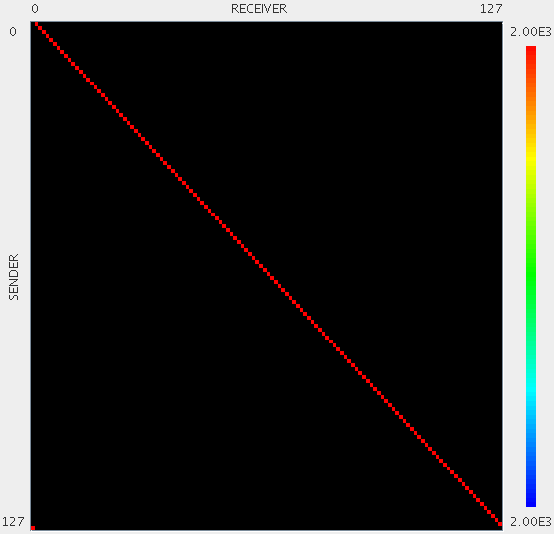
\includegraphics[width=.82\linewidth]{tau-comm-matrix}
        \caption{TAU}%
        \label{fig:tau-comm-matrix}
    \end{subfigure}
    \begin{subfigure}{.49\linewidth}
        \centering
        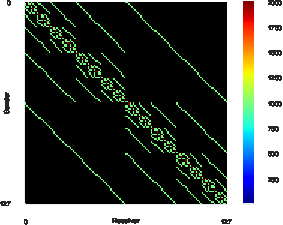
\includegraphics[width=.99\linewidth]{pfprof-comm-matrix}
        \caption{PFProf}%
        \label{fig:pfprof-comm-matrix}
    \end{subfigure}
    \caption{Extracted Communication Patterns}%
    \label{fig:profiler-comparison}
\end{figure}

\subsection{Accuracy of Traffic Estimated by PFSim}%
\label{sec:ii-eval-pfsim}

This experiment evaluates the accuracy of the simulation performed with PFSim.
The traffic estimated by PFSim and the traffic measured when running an
application on an actual cluster are compared.

The simulated cluster was modeled after a small-scale cluster installed at our
institution. The cluster is composed of 20 compute nodes, each equipped with
two quad-core Intel Xeon E5520 processors. Compute nodes are interconnected
with a two-tier fat-tree topology as illustrated in
Fig.~\ref{fig:cluster-config}. A single NEC ProgrammableFlow PF5240 switch is
logically divided into six switches that constitute the fat-tree topology.
The upper-layer two switches are referred to as spine1--spine2 and the
lower-layer four switches as leaf1--leaf4. The CG benchmark from the
NAS Parallel Benchmark Suite~\autocite{Bailey1991} was executed with 128
processes on 16 compute nodes. Since the CG benchmark only allows power-of-two
number of processes, some compute nodes could not be utilized.

\begin{figure}
    \centering
    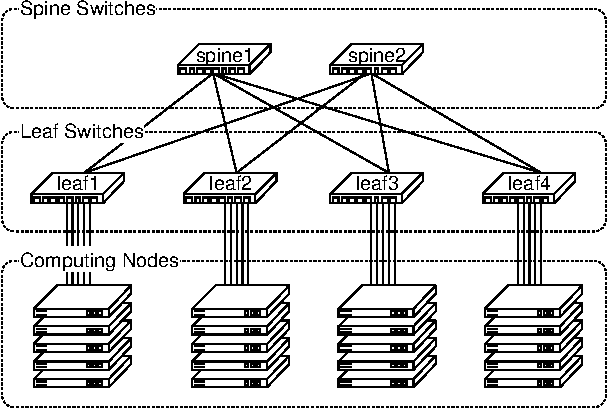
\includegraphics{pfsim-eval-cluster}
    \caption{Simulated Cluster with Fat-tree Interconnect}%
    \label{fig:cluster-config}
\end{figure}

Figure~\ref{fig:pfsim-accuracy} shows the comparison of simulated traffic
using PFSim and the measured traffic on the original cluster. The traffic on
each link between the spine switches and leaf switches were normalized by the
traffic on the link spine1$\rightarrow$leaf1 and shown in the plot. The plot
indicates the error of simulation result is small. The largest error was 1.9\%
and was observed on the link leaf4$\rightarrow$spine1. These results indicate
that the simulation result is sufficiently accurate to analyze performance of
dynamic interconnects.

\begin{figure}
    \centering
    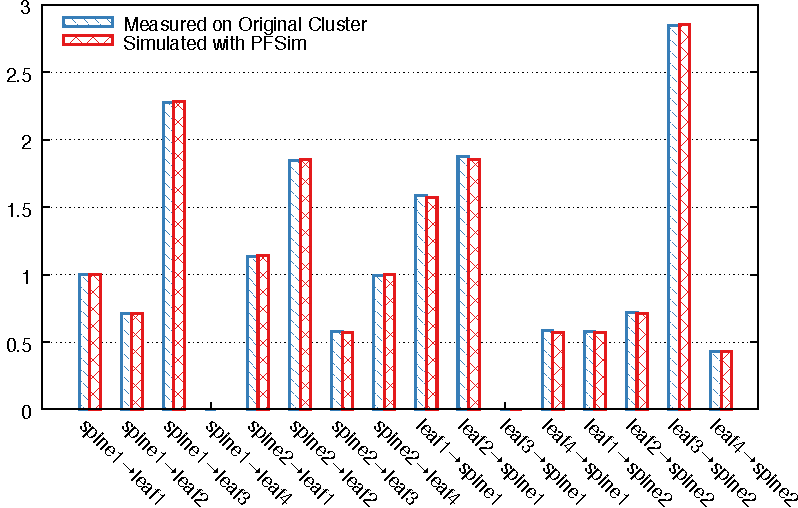
\includegraphics{pfsim-accuracy}
    \caption{Comparison of Simulated Traffic against Measured Traffic}%
    \label{fig:pfsim-accuracy}
\end{figure}

\subsection{Overhead Incurred by PFProf}

In this experiment, the performance of point-to-point communication
between two processes with and without PFProf were compared to inspect
the overhead incurred by the profiler. OSU Micro
Benchmark~\autocite{omb} was used to measure the throughput and latency
of point-to-point communication between two processes for varying
message sizes. The comparison of throughput and relative throughput are shown
in Fig.~\ref{fig:pfprof-bw-abs} and Fig.~\ref{fig:pfprof-bw-abs},
respectively. For messages larger than 1KB, the overhead was ignorable. For
messages smaller than 1KB, up to 30\% of overhead was incurred. Comparison of
latency and relative latency are shown shown in Fig.~\ref{fig:pfprof-lat-abs}
and Fig.~\ref{fig:pfprof-lat-rel}, respectively. These plots suggest that
there is almost no overhead for latency. These results indicate that PFProf is
able to extract the communication pattern from applications without
significantly hurting the performance of applications.

\begin{figure}
    \centering
    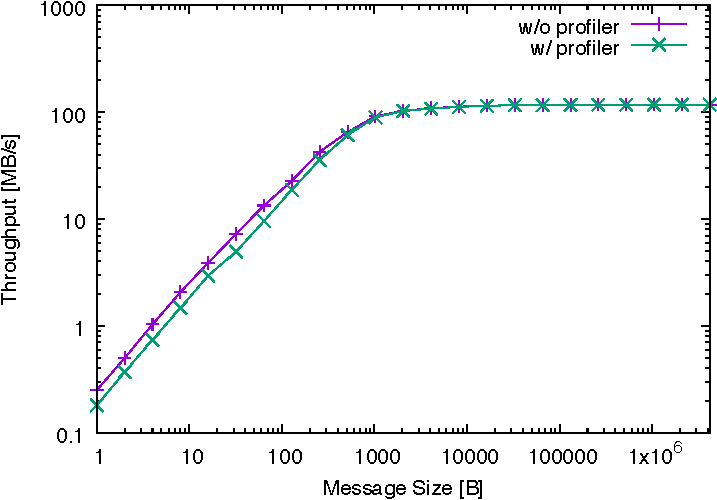
\includegraphics{pfprof_bandwidth_abs}
    \caption{Throughput of Point-to-point Communication}%
    \label{fig:pfprof-bw-abs}
\end{figure}

\begin{figure}
    \centering
    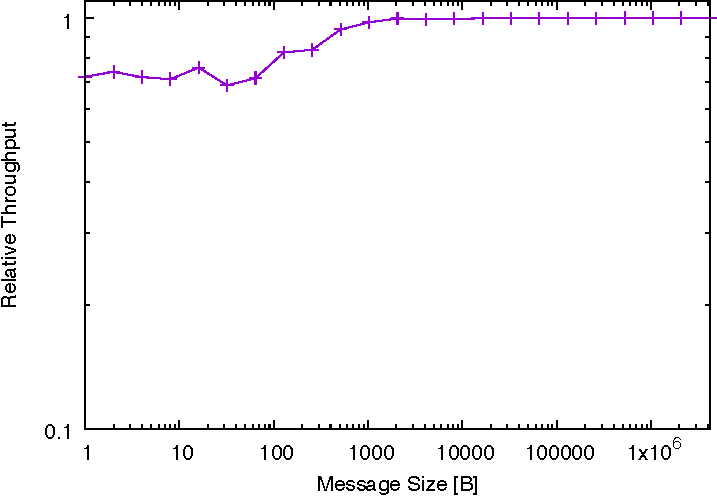
\includegraphics{pfprof_bandwidth_rel}
    \caption{Relative Throughput of Point-to-point Communication}%
    \label{fig:pfprof-bw-rel}
\end{figure}

\begin{figure}
    \centering
    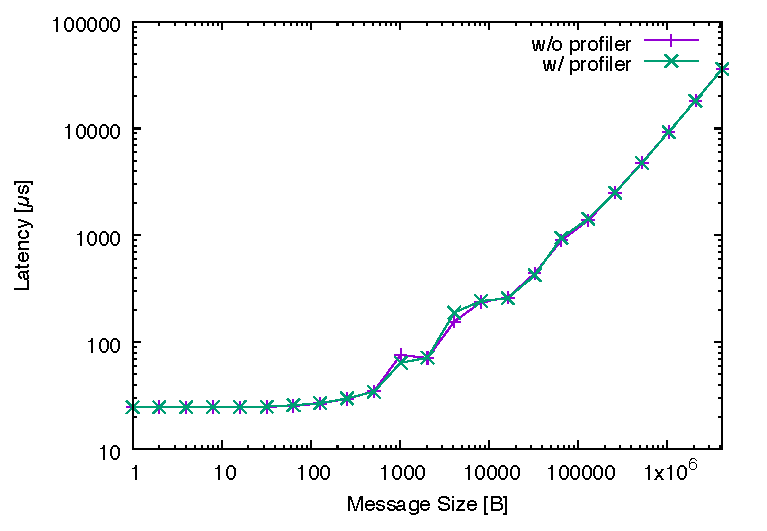
\includegraphics{pfprof_latency_abs}
    \caption{Latency of Point-to-point Communication}%
    \label{fig:pfprof-lat-abs}
\end{figure}

\begin{figure}
    \centering
    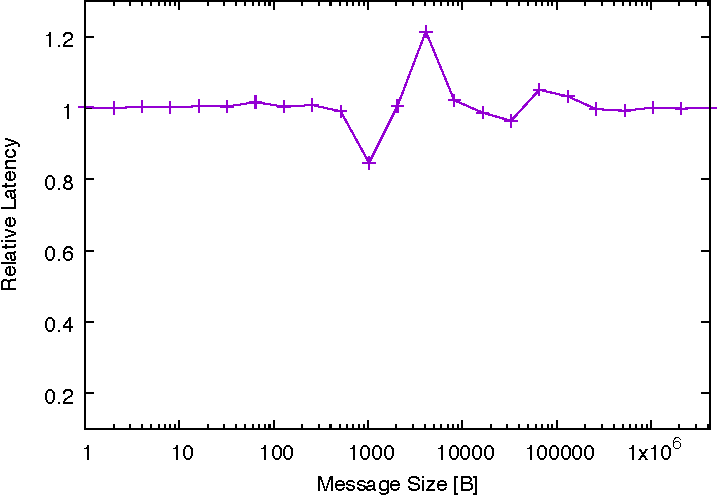
\includegraphics{pfprof_latency_rel}
    \caption{Relative Latency of Point-to-point Communication}%
    \label{fig:pfprof-lat-rel}
\end{figure}

\subsection{Use Case of PFAnalyzer}\label{sec:ii-simulation-results}

This experiment shows how PFAnalyzer can be used by researchers to analyze the
joint effect of node allocation, process placement and routing on the
distribution of traffic in the interconnect. Communication-intensive MPI
applications were executed on the proposed simulator. The maximum traffic load
observed on links composing the interconnect was compared in both cases of
static interconnect control and dynamic interconnect control. The maximum
traffic load observed on the links was used as an indicator of the
communication performance of an application. In most cases, a hot spot link
can slow down the whole application, because every process needs to wait until
the slow communication crossing the hot spot link completes when collective
communication or synchronization is performed by an application. Therefore,
mitigating the traffic load on the hot spot link is considered to improve the
performance of the application.

Two applications were selected as representatives of communication-intensive
applications. The first one was the CG benchmark from the NAS Parallel
Benchmark Suite~\autocite{Bailey1991}. The CG benchmark estimates the largest
eigenvalue of a sparse matrix using the inverse power method. Internally it
uses the conjugate gradient method, which frequently appears in irregular mesh
applications. The second application (\lstinline!ks_imp_dyn!) was from MIMD
Lattice Computation (MILC)~\autocite{milc}, a collection of applications used
to study Quantum Chromodynamics (QCD). As for the input data, the data set
provided by NERSC as a part of the NERSC MILC benchmark was used. These two
applications were executed with 128 MPI processes. Thread parallelism was not
put in use (\emph{i.e.,} flat MPI model was adopted).

To analyze the effect of dynamic interconnect control, simulations were
carried out using static routing and dynamic routing control. Furthermore, in
order to investigate the impact of node selection and process placement to the
traffic load, the node selection algorithm and process placement algorithm
were also changed. As a result, exhaustive combinations of two node selection
algorithms, two process placement algorithms and two routing algorithms were
investigated with the scheduling algorithm fixed. Below are the descriptions
of the algorithms used in this experiment:

\begin{itemize}
\item
  Scheduling: A simple \emph{First-Come First-Served (FCFS)} scheduling
  without backfilling was adopted.
\item
  Node Selection: Either \emph{linear} or \emph{random} node selection
  was adopted. Linear node selection assumes that compute nodes are
  lined up in a one-dimensional array and minimizes the fragmentation of
  allocation. This is essentially the same as the default node selection
  policy of Slurm~\autocite{Yoo2003}. Random node selection, as the name
  indicates, randomly selects compute nodes. This algorithm simulates a
  situation where the allocation of compute nodes is highly fragmented.
\item
  Process Placement: Either \emph{block} or \emph{cyclic} process
  placement was adopted. Block process placement assigns rank \(i\) to
  the \(\lfloor i / c \rfloor\)-th compute node where \(c\) represents
  the number of cores per node. Cyclic process placement assigns rank
  \(i\) to the \((i \bmod n)\)-th compute node where \(n\) denotes the
  number of compute nodes.
\item
  Routing: Either \emph{D-mod-K} routing or a \emph{dynamic} routing was
  adopted. Destination-modulo-K (\mbox{D-mod-K}) routing is a
  popular static load balancing routing algorithm that distributes
  packet flow over multiple paths based on the destination address of
  the packet. The dynamic routing algorithm implemented here computes
  and allocates routes from the heaviest communicating process pair. A
  route is computed to minimize the traffic of the maximum-traffic link
  in the path.
\end{itemize}

Under this condition, the maximum traffic load observed on links through the
simulation were measured and compared.
Figure~\ref{fig:nas-cg-congestion} shows the simulation results in
the NAS CG benchmark. In this graph, the blue hatched bars represent the
results for \mbox{D-mod-K} routing while the red crosshatched bars represent
the results for dynamic routing. The vertical axis represents the simulated
maximum traffic load normalized by the maximum traffic load when linear node
selection, block process placement and \mbox{D-mod-K} routing were adopted.

What stands out in Fig.~\ref{fig:nas-cg-congestion} is that
dynamic routing consistently achieves lower traffic load compared to
static \mbox{D-mod-K} routing. The reduction of traffic load was the largest
when linear node selection and block process placement were adopted. Under
this combination of node selection and the process placement algorithm,
dynamic routing slashed the maximum traffic load by 50\% in comparison with
\mbox{D-mod-K} routing. Also, the graph reveals that cyclic process
placement always increased maximum traffic load compared to block process
placement because neighboring ranks were placed on different compute nodes
despite the locality of the communication pattern.

\begin{figure}
    \centering
    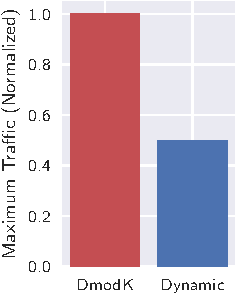
\includegraphics{nas_cg_congestion}
    \caption{Comparison of Maximum Traffic (NAS CG)}%
    \label{fig:nas-cg-congestion}
\end{figure}

\begin{figure}
    \centering
    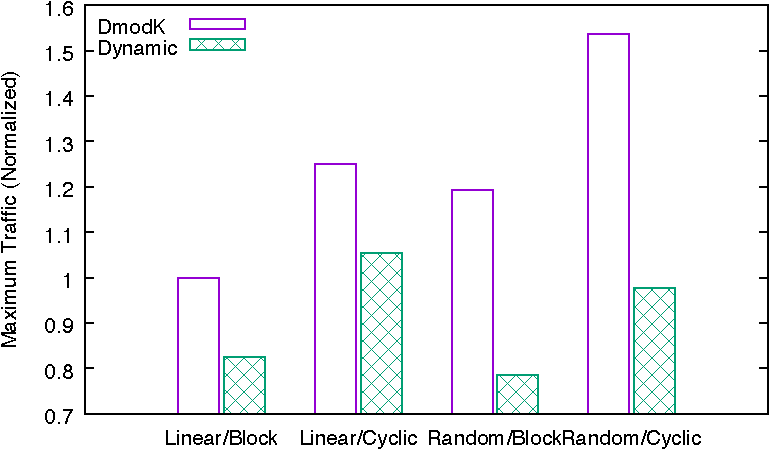
\includegraphics{nersc_milc_congestion}
    \caption{Comparison of Maximum Traffic (MILC)}%
    \label{fig:nersc-milc-congestion}
\end{figure}

Figure~\ref{fig:nersc-milc-congestion} shows the result in the case of
MILC\@. The graph reveals that dynamic routing outperforms \mbox{D-mod-K}
routing. In this case, the reduction of the link load was the largest when
random node selection and cyclic process placement was adopted. When using
linear node selection and block process placement, the reduction of the
maximum link load was 18\%. Compared to NAS CG benchmark, the effect of
dynamic routing was smaller.

To investigate the impact of traffic load on the application performance of an
actual environment, the configuration described in the previous
Section~\ref{sec:ii-simulation-results} was reproduced on a actual cluster and
then the execution time of each benchmark was measured. This cluster was
equipped with switches that support OpenFlow, which is a de facto standard
implementation of SDN\@. The routing algorithms were implemented based on
OpenFlow. In this experiment, linear node selection and block process
placement was adopted. The average execution time of 10 runs was compared when
using \mbox{D-mod-K} routing and dynamic routing. Figure~\ref{fig:cg-nersc-time}
shows the measured execution time for both benchmarks. The use of dynamic
routing reduced the execution time of NAS CG benchmark for 23\%. Meanwhile,
the execution time of MILC benchmark was reduced for 8\%, which was smaller
than the case of NAS CG benchmark. This matches with the simulation result
that predicted NAS CG benefits from larger reduction in maximum traffic load
by using dynamic routing compared to MILC\@.

These results suggest that application performance is actually improved
by alleviating the traffic load on the hot spot link. This suggestion
implies that researchers working on dynamic interconnects can take advantage
of the proposed toolset to simulate different packet flow controlling
algorithms and assess their performance improvement effect on real-world
applications by using indicators such as maximum traffic load.

\begin{figure}
    \centering
    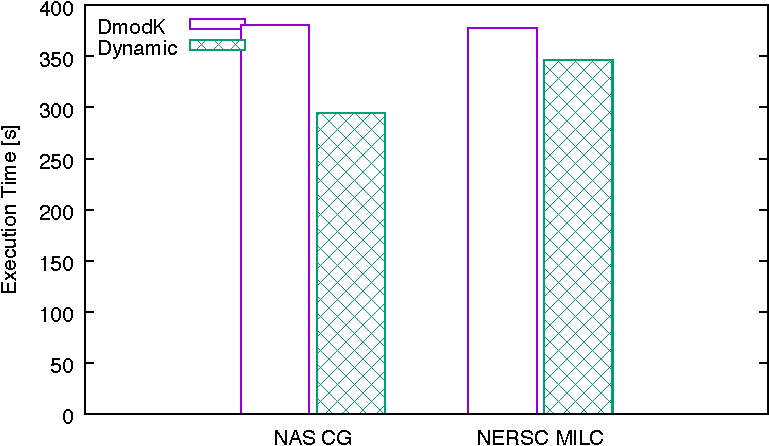
\includegraphics{pfsim_exec_time}
    \caption{Comparison of Execution Time on an Actual Cluster}%
    \label{fig:cg-nersc-time}
\end{figure}

\section{Related Work}\label{sec:ii-related-work}

Several interconnect simulators have been proposed in the past research.
PSINS~\autocite{Tikir2009} is a trace-driven simulator for HPC
applications. Traces obtained from applications are used to predict the
performance of applications on a variety of HPC clusters with different
configurations. LogGOPSim~\autocite{Hoefler2010} simulates the execution
of MPI applications based on the LogGOP network model. A limitation of
LogGOPSim is that the interconnect is assumed to have full bisection bandwidth
and thus congestion is not simulated. These two simulators can provide
accurate performance predictions owing to their per-message simulation
capability. However, the topology and the routing algorithm of interconnects
are abstracted in the network models of PSINS and LogGOPSim. Therefore, these
simulators cannot be used for predicting and comparing the performance of
different topologies or routing algorithms. In contrast, the simulator
proposed in this chapter allows users to compare the performance
characteristic of different topologies and routing algorithms.

ORCS~\autocite{Schneider2009} simulates the traffic load on each link in
the interconnect for a given topology, communication pattern and routing
algorithm in the same way as PFSim. The simulated traffic load of links can be
summarized into various performance metrics and used for further analysis. A
limitation of ORCS is that only pre-defined communication patterns can be used
as its input. Moreover, ORCS assumes static routing as in InfiniBand. On the
contrary, PFSim can handle dynamic routing algorithms that use communication
patterns of applications and interconnect usage to make routing decisions.

In~\autocite{Jo2015}, simulations are carried out to examine the
performance characteristics of an SDN-based multipath routing algorithm
for data center networks. A simulator was developed based on MiniSSF to
simulate the throughput and delay of a packet flow under diverse
settings. However, communication patterns are randomly generated and not
based on real-world applications. PFSim is designed to accept arbitrary
communication patterns obtained from real-world applications using our custom
profiler.

\(\mathit{INAM}^2\)~\autocite{Subramoni2016} is a comprehensive tool to
monitor and analyze network activities in an InfiniBand network. The
tight integration with the job scheduler and a co-designed MPI library
allows \(\mathit{INAM}^2\) to associate network activities with jobs and
MPI processes. For instance, it can identify hot spots in the
interconnect and inspect which node, job, and process is causing the
congestion. Although \(\mathit{INAM}^2\) is a useful tool for system
administrators to diagnose the performance issues of interconnects, it
is not suitable for studying diverse interconnects since it only
supports physical clusters.

\section{Conclusion}\label{sec:ii-conclusion}

This chapter described the design and implementation of PFAnalyzer, a
toolset for analyzing the performance characteristics of
application-aware dynamic interconnects. PFAnalyzer is composed of
PFProf, a profiler to extract communication patterns from applications,
and PFSim, a simulator capable of simulating application-aware dynamic
interconnects. PFSim takes a set of communication patterns of
applications and a cluster configuration as its input and then simulates
the traffic on each link of the interconnect. Evaluation conducted in this
dissertation verified that PFProf is able to capture the underlying
point-to-point communication of collective communication, which is essential
for understanding the communication characteristic of applications. Also, it
also indicated that the incurred overhead is small. Furthermore, the error of
traffic simulated with PFSim was 1.9\% at maximum, which is small enough to
analyze the performance characteristic of interconnects.

PFAnalyzer contributes to realizing a programmable interconnect control
adaptive to the communication pattern of application in two aspects. First,
PFProf allows researchers to accurately extract the inter-process
communication pattern from applications. The obtained communication pattern is
a crucial information for understanding the communication characteristic of
applications and adapting the interconnect control to the application. Second,
PFSim helps researchers to design and implement effective algorithms to
control the packet flow in the interconnect for mitigating imbalance in the
interconnect and achieving higher communication performance between compute
nodes.

Further work is necessary to investigate the performance characteristics of
dynamic interconnects on large-scale and highly parallel clusters. Moreover,
application-aware node selection and process placement algorithms are planned
to be implemented on PFSim. The impact of such application-aware algorithms on
the performance of dynamic interconnects should be evaluated.

\chapter{Accelerated MPI Collective Using Software-Defined Networking}\label{sec:iii}

\section{Introduction}\label{sec:iii-introduction}

As described in Section~\ref{sec:i-mpi}, communication primitives defined in
MPI can be roughly categorized into point-to-point communication, collective
communication and one-sided communication. Out of these three categories, this
dissertation particularly focus on accelerating collective communication
because of its significant impact to the application performance. In fact, a
recent analysis of MPI usage on a production HPC system has revealed that
approximately 34\% of the total core-hours of the system are expended in MPI
communication and 66\% of the total MPI communication time is spent in
collective communication~\autocite{Chunduri2018}. This fact clearly indicates
that reducing the time of collective communication is of great importance.

MPI collectives require intensive communication among multiple compute node
pairs. However, some compute node pairs communicate less, whereas other pairs
have to communicate much more. Because of this imbalance, even in the case
where the interconnect of a cluster system has multiple redundant routes
between compute nodes, the packet flow generated from MPI collectives could
collide on a single link of the interconnect without any control of packet
flow.

This chapter aims at accelerating MPI collectives by dynamically controlling
the packet flow in the interconnect. In particular, a cluster system deployed
with an interconnect that contains multiple redundant routes is targeted. This
is because the majority of interconnects today are provisioned with redundant
routes to improve the bisection bandwidth and fault tolerance. Specifically,
this research specifically focuses on fat-tree. This research designs and
implements a framework that effectively makes use of redundant routes by
dynamically controlling the packet flow in the interconnect using SDN
described in Section~\ref{sec:i-sdn}.

The rest of this chapter is organized as follows.
Section~\ref{sec:iii-background} reviews conventional traffic balancing
methods and analyzes their problems. Subsequently, the goal of this chapter is
clarified. In Section~\ref{sec:iii-proposal}, the design and implementation of
the proposed architecture of SDN-enhanced MPI\_Allreduce is presented. In
Section~\ref{sec:iii-evaluation}, an evaluation on a cluster system is
conducted to verify the feasibility of the proposed framework.
Section~\ref{sec:iii-related-work} discusses related works.
Section~\ref{sec:iii-conclusion} concludes this chapter and discusses
challenges for further improving the practicality of our proposed framework.

\section{Research Objective}\label{sec:iii-background}

MPI collective operations require a large number of simultaneous communication
among multiple process pairs. However, some compute node pairs communicate
less, whereas other pairs have to communicate much more. When the underlying
network of the cluster system that interconnects with the compute nodes has a
full-bisection bandwidth, the imbalance of source and destination in
communication would not be a problem although structuring this type of a
network is hard to scale out due to economic and physical
restrictions~\autocite{Al-Fares2008}. Under the assumption that the network is
oversubscribed, the shortage of available bandwidth could give rise to a
serious problem.

Suppose a cluster system of four compute nodes interconnected with a
two-tier fat-tree topology as illustrated in Fig.~\ref{fig:problem-routing1}.
Fat-tree is a network topology that has multiple redundant routes between the
upper layer switches and lower layer switches. By distributing traffic among
these redundant routes, it is possible to gain higher bisection bandwidth
compared to a simple tree topology.

The traffic load balancing algorithm deployed on the interconnect becomes
important on such an interconnect. For example, suppose compute node 1 is
sending data to node 3, and node 2 is sending different data to node 4 at the
same moment in Fig.~\ref{fig:problem-routing1}. If those two communications
are routed within the exact same route, link contention could happen. When
these two communications are routed so that they make use of the redundant
routes as depicted in Fig.~\ref{fig:problem-routing2}, link contention can be
avoided.

\begin{figure}
    \centering
    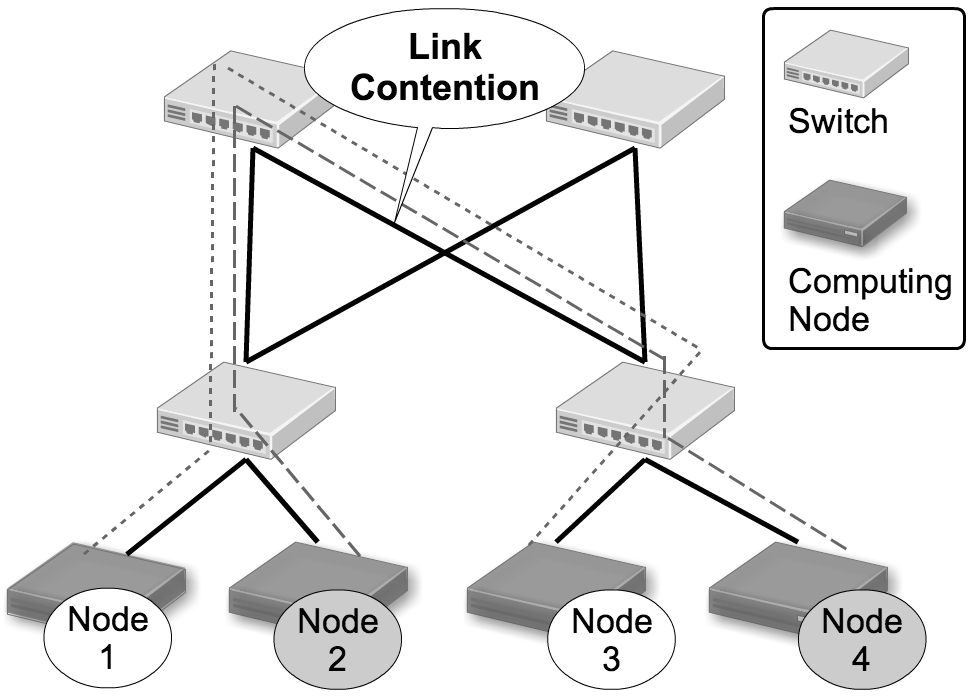
\includegraphics[width=.6\linewidth]{problem-routing2.png}
    \caption{Link Contention on Fat-tree}%
    \label{fig:problem-routing1}
\end{figure}

\begin{figure}
    \centering
    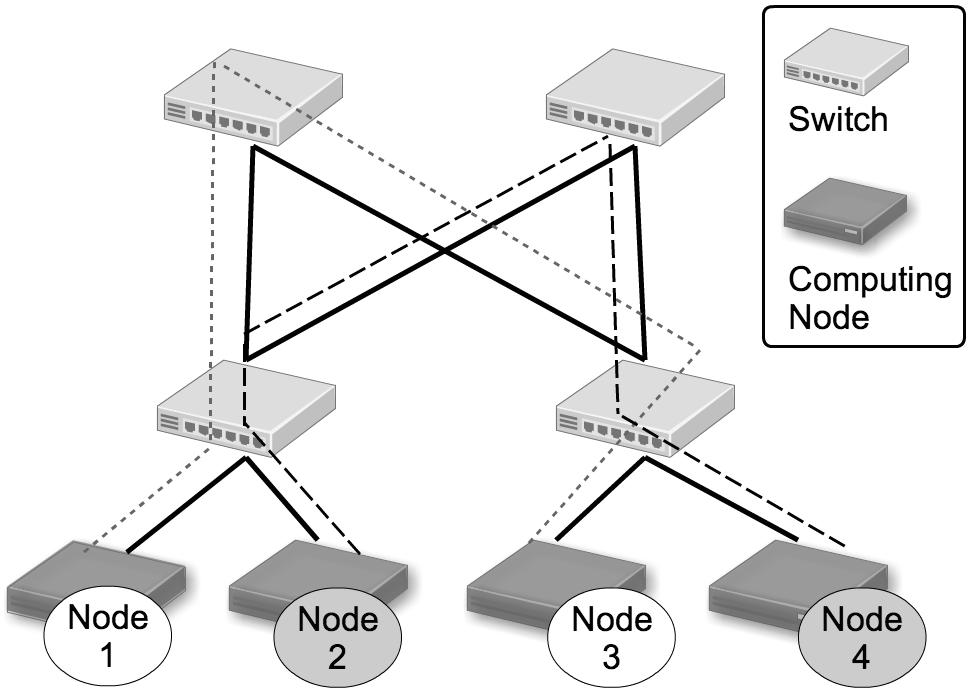
\includegraphics[width=.6\linewidth]{problem-routing1.png}
    \caption{Load Balancing Routes on Fat-tree}%
    \label{fig:problem-routing2}
\end{figure}

Various algorithms for balancing traffic in a network with redundant routes
have been proposed. Equal-Cost Multi-Path routing (ECMP)~\autocite{ecmp} is a
standardized load balancing strategy mainly used in L3 switches. For each
communication between two compute nodes, if multiple equal cost routes are
available, ECMP selects one route from among them. The decision on which route
to use is based on the header fields (\emph{e.g.} source and destination
addresses) of each packet. A hash function is applied to the header fields to
generate the corresponding hash value for the header fields, where every value
in the hash value space are evenly assigned to one of the equal cost routes.

InfiniBand~\autocite{Buyya2009} is a computer network communication link
commonly used in the area of HPC and a data center. InfiniBand supports
multiple routing methods. One of those methods is a min-hop routing
algorithm, which calculates the minimum hop route between every
compute node pair. If multiple minimum hop routes for a single
compute node pair are available, the algorithm assigns a route so that
usage among links is equalized.

The problem of these existing conventional load balancing mechanisms is
that they never consider the communication pattern of MPI applications. In
general, MPI applications cannot retrieve the usage information of the
underlying network nor control it. Meanwhile, MPI communication in an MPI
application usually shows a strong locality where each process communicates
with a limited number of processes. This non-uniform communication pattern may
cause an inequality of link usage that decreases available bandwidth between
compute nodes. Ultimately, this decrease of available bandwidth can lead to
the performance degradation of MPI applications.

From the observations above, an application-aware network control mechanism
which recognizes the communication pattern needed by MPI collectives is
essential. Also, the mechanism must effectively utilize the bandwidth of each
link by distributing the traffic among redundant routes. Therefore, this
research leverage Software-Defined Networking (SDN) to enable such dynamic
control of packet flow depending on the communication patterns of MPI
applications.

In particular, this research focuses on accelerating MPI\_Allreduce.
MPI\_Allreduce is one of the most frequently used and time-consuming
collective communication functions of MPI\@~\cite{Chunduri2018}.
This collective communication reduces values from all
processes with an operator and broadcasts the result of the reduction to every
process. More specifically, suppose there are $n$ processes in a communicator
and each process with rank $i$ ($0 \leq i < n$) has $l$ values $x_i^0, x_i^1,
\dots, x_i^l$. After MPI\_Allreduce is completed, all processes have values
$y^0, y^1, \dots, y^l$ where $y^j = x_0^j \oplus x_1^j \oplus \dots \oplus
x_{n-1}^j$ and $\oplus$ is the operator used for reduction. The operator can
be any user-defined associative operator or one of the pre-defined operators
such as sum, product, or maximum. Figure~\ref{fig:mpi-allreduce} shows an
example where four processes each having five values call MPI\_Allreduce with
the sum operator.

\begin{figure}
    \centering
    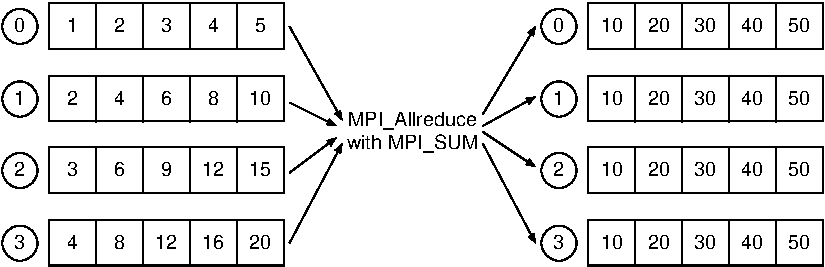
\includegraphics{mpi-allreduce}
    \caption{Effect of MPI\_Allreduce}%
    \label{fig:mpi-allreduce}
\end{figure}

One of the use cases of MPI\_Allreduce is parallel Conjugate Gradient~(CG)
method. CG method is an iterative algorithm to solve a system of linear
equations $Ax = b$ whose coefficient matrix $A$ is positive-definite and
symmetric. In the parallel CG method, a significant amount of time is spent in
MPI\_Allreduce to compute the inner product of
vectors~\autocite{Kandalla2012}. Another use case is parallel Stochastic
Gradient Descent~(SGD). SGD is a continuous optimization algorithm that
minimizes an objective function $f$ parameterized by $w$ for a given set of
input $S$. SGD incrementally updates $w$ in the following way: $w^{t+1}=w^t-
\eta \nabla f(w^t; z^t)$ where $w^t$ is the parameter for the $t$-th
iteration, $z^t$ is an input data randomly sampled from $S$, and $\eta$ is a
small constant. In parallel SGD, the gradient $\nabla f(w^t; z^t)$ is computed
in parallel by each process using different samples. Subsequently,
MPI\_Allreduce is used to compute the average of the individual gradients
computed by all processes.

This research attempts to accelerate MPI\_Allreduce on a cluster system with a
fat-tree interconnect. The dynamic network controllability of SDN is
integrated with MPI in order to mitigate link contention. The speedup of
MPI\_Allreduce based on the proposed framework is evaluated.

\section{Proposal}\label{sec:iii-proposal}

This section presents the proposed framework for accelerating MPI collectives.
First, the basic idea behind the proposed framework is outlined. After that,
the design and implementation of the framework is described in detail.

\subsection{Basic Idea}

The motivation behind the proposed framework is to improve the inefficient communication
in MPI in order to enhance the performance of MPI applications. The fact that
MPI applications are unable to retrieve the usage of the underlying network
results in a potential inefficiency in terms of communication. One of such
inefficiencies is the inequality of link usage among links. Since the
bandwidth of a link is limited, an inequality of link usage can cause
congestion in heavy-loaded links. Therefore, this research focuses on the
inequality of the link usage among the interconnect of a cluster system.

In this chapter, redundant routes in the interconnect are used to mitigate the
inequality of link usage, based on an assumption that the cluster system has a
fat-tree interconnect. Through this traffic distribution, contention in the
links is expected to be alleviated, which as a result speeds up communication.

\subsection{Design of Collective Acceleration Framework Using SDN}%
\label{sec:iii-design}

The proposed framework is composed of three modules. These three modules are
SDN controller, LLDP~(Link Layer Discovery Protocol)~\autocite{lldp} daemon
and SDN MPI library. They are deployed onto a cluster system as illustrated in
Fig.~\ref{fig:proposal-placement}. The SDN controller is designed to be
deployed onto the management node of a cluster system. The management node is
used for controlling the whole cluster system such as deploying jobs to the
system. The LLDP daemon is designed to run in the background on all compute
nodes. The SDN MPI library is a library that needs be statically linked to MPI
applications at compile time.

Although each compute node can run one or more MPI processes, in this chapter,
it is assumed that each compute node runs only a single MPI process. This is a
reasonable assumption since many applications nowadays leverage \emph{hybrid
parallelism}, which combines distributed memory programming and shared memory
programming. Under the hybrid parallelism model, the application starts a
single MPI process per node and then spawns a thread for each socket or core
on the node. After that, the application uses MPI for intra-node communication
and threading frameworks such as OpenMP for intra-node communication.

\begin{figure}
    \centering
    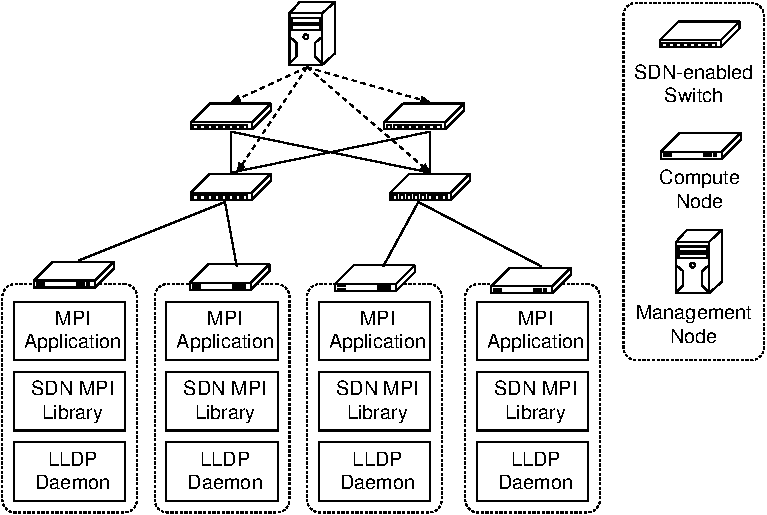
\includegraphics{sdn-mpi-arch}
    \caption{Placement of the Modules Composing SDN-enhanced MPI\_Allreduce}%
    \label{fig:proposal-placement}
\end{figure}

The interaction among these modules is roughly divided into two phases: the
initialization phase at the MPI application startup and the main phase at each
MPI collective call. Figure~\ref{fig:proposal-sequence} is a UML sequence
diagram that illustrates how these modules cooperate with each other.
MPI\_Init is the MPI function that initializes the MPI execution environment,
which must be called on the application startup. After MPI\_Init finishes, all
MPI processes notify their own IP address and MPI rank number to the SDN
controller. This information obtained from MPI processes is held by the
controller until the execution of the MPI application finishes.

\begin{figure}
    \centering
    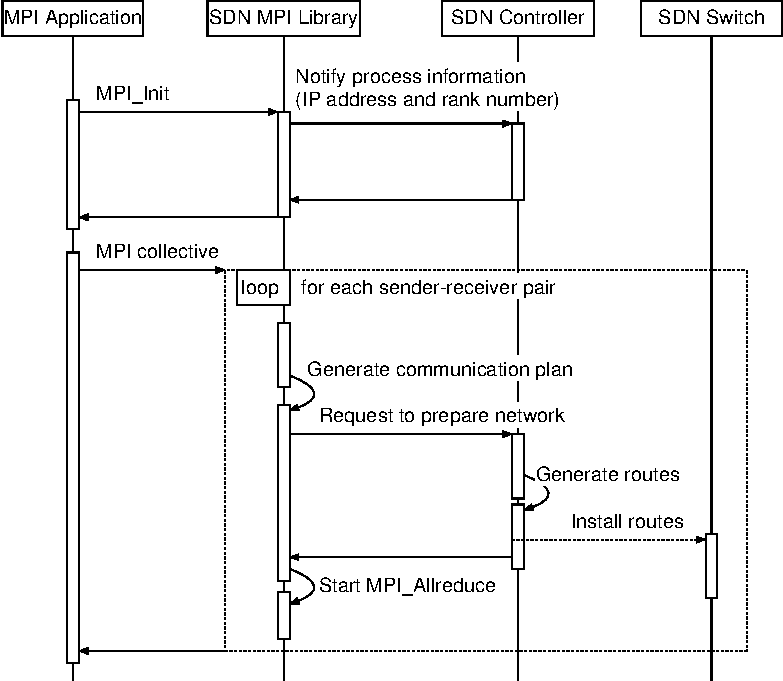
\includegraphics{sdn-mpi-sequence}
    \caption{The Sequence Diagram of the Proposed Framework}%
    \label{fig:proposal-sequence}
\end{figure}

When an MPI collective is called, the rank 0 process generates the
communication pattern of the MPI collective. This communication pattern is a
set of sender process and receiver process pairs during the MPI collective
communication. After the communication pattern is generated, this set is sent
to the SDN controller by the rank 0 process. As soon as the SDN controller
receives the communication pattern, it generates a route for each
sender-receiver pair. Subsequently, the SDN controller programs each
SDN-enabled switch so that the MPI packets are routed along the pre-generated
routes. After the entire communication pattern is processed, the MPI
collective is called to start the actual data transfer and computation for the
collective operation.

\subsection{Implementation of Collective Acceleration Framework Using SDN}

To realize the proposed framework, three modules that work as an integrated
system has been developed: LLDP daemon, SDN controller and SDN MPI library.
This section explains the implementation of these three modules in detail.

\subsubsection{LLDP Daemon}

Each compute node runs an LLDP daemon in the background. This daemon is
designed to emit LLDP packets containing hardware information periodically,
which are received by the SDN-enabled switches and used for topology
discovery. Some LLDP daemon implementations already exist. However, a new,
minimal daemon has been developed to easily add and tweak features so that it
can cooperate with the other programs composing the whole system.

The developed daemon detects all available network interfaces installed on a
computer and queries its interface index, MAC address and IP address.
This information is packed into a single LLDP packet and sent out from
each network interface periodically. The interval is set to one second in
this prototypical implementation to speed up the topology discovery.
However, it can be a longer period in practical systems so that its
topology does not change frequently.

As described above, the LLDP daemon emits a few hundred byte long packets to
the network every second. This traffic is considered to be small enough so
that it does not cause serious side effects on the actual MPI process, for
instance taking CPU time away from the application or consuming too much
bandwidth that could interfere with the MPI communication. Generating such
LLDP packets is also not a difficult task for a today's  computer, so the
impact to the application is considered to be ignorable.

\subsubsection{SDN Controller}

The SDN controller was developed on top  of Trema~\autocite{trema}, a
framework designed for easily developing OpenFlow controllers in the Ruby
language. It has the following four core functionalities:

\begin{enumerate}
    \item Generating routes for MPI collectives to mitigate link contention
          and installing the generated routes to SDN-enabled switches
    \item Detecting the topology and usage of the interconnect using LLDP
    \item Responding to Address Resolution Protocol~(ARP) requests from
          compute nodes to avoid broadcast storms
    \item Routing of non-MPI traffic such as ICMP and SSH
\end{enumerate}

The first functionality is topology detection. How detection is
performed is shown in Fig.~\ref{fig:lldp}. The controller periodically
requests every switch to send out an LLDP packet from each of their physical
ports (step~1 in Fig.~\ref{fig:lldp}). This LLDP packet contains two kinds of
information: datapath ID (a number that uniquely distinguishes the switches)
and port number (port index where the packet is sent out). Moreover, all
compute nodes also emit LLDP packets from the LLDP daemon described in the
previous section. The controller is notified of a LLDP packet arrival at a
switch. After that, it parses the packet to obtain the information on the
packet's origin, and then examines whether the packet came from a compute node
or an SDN-enabled switch. If the sender is a compute node, its MAC address and
interface index is acquired. Otherwise if the sender is a switch, its datapath
ID and port number is acquired (step~2). Using this information from its
neighbors, an adjacency list is generated (step~3). From this adjacency list,
a network topology graph is constructed, which is used in the route generation
and routing. If the packet is from a compute node, the source MAC address and
IP address are registered in a MAC/IP address translation table used in the
ARP responding functionality.

\begin{figure}
    \centering
    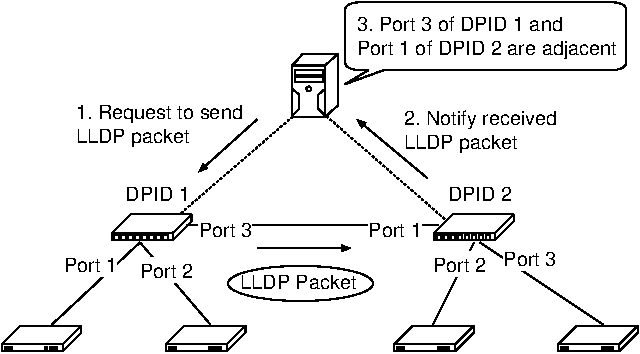
\includegraphics{lldp}
    \caption{Topology Detection using LLDP}%
    \label{fig:lldp}
\end{figure}

The second functionality is replying to ARP requests. ARP requests are L2
broadcast packet and therefore causes a \emph{broadcast storm} in a network
that contains a cycle. Since this chapter targets a network that has redundant
routes, the topology of the network is not a tree. Therefore, the network is
always cyclic. Thus, the controller instructs the switches to reply to the
received ARP request, instead of the compute node that has the corresponding
IP address. The IP address that corresponds to the MAC address is obtained
from the MAC/IP address translation table described above.

The third functionality is route generation and installation for MPI
collective communication. The route generation algorithm is implemented as a
pluggable module so that different algorithms can be specifically tailored for
each MPI collective.

% アルゴリズムの目的
Since this research focuses on accelerating MPI\_Allreduce, a route generation
algorithm targeting MPI\_Allreduce has been designed and implemented. The goal
of this route generation algorithm is to mitigate the interference between the
packet flows generated by the underlying point-to-point communication of
MPI\_Allreduce. In particular, the proposed algorithm tries to generate routes
so that the packet flows are evenly distributed among the redundant routes in
the interconnect. In other words, the proposed algorithm aims to minimize the
maximum number of packet flows sharing a link.

% 解の最適性についての議論
Note that this problem is a combinatorial optimization problem on a
multi-commodity flow network and thus requires heavy computation to find the
optimal solution. Meanwhile, the SDN controller needs to perform the route
generation every time an MPI collective is called as described in
Section~\ref{sec:iii-design}. Therefore, the proposed algorithm is designed to
be a heuristic algorithm based on a greedy strategy that quickly finds an
approximate solution rather than an optimal solution.

% アルゴリズムの基本的なアイディア
The basic idea behind this heuristic algorithm is to assign a route to each
point-to-point communication iteratively. At each iteration, the algorithm
selects a pair of a sender and a receiver and finds the least utilized route
between them. This is achieved by considering a weighted graph where the
weight of a link is equal to the total number of packet flows going through
the link, and then finding the shortest route between the sender process and
receiver process in this graph. Here, the \emph{Dijkstra} algorithm is used to
find the shortest route because of its speed and simplicity. After a route is
assigned, the weight of each link along the generated route is incremented.
This procedure is repeated for all sender-receiver pairs.

% 擬似コードを使った具体的な説明
Algorithm~\ref{lst:code-generate-route} is a pseudo-code for the algorithm.
First, an empty array \emph{routes} is initialized (line 1 in
Algorithm~\ref{lst:code-generate-route}). After that, the route search is
performed for each sender-receiver pair (line 4--7). The resulting route is
added to \emph{routes} (line 5) and the link weight (which is the number of
total routes that use that link) of each link is incremented (line 6--7).
After all routes are generated, these routes are installed to the SDN-enabled
switches.

\begin{algorithm}
    \SetKwData{Routes}{routes}
    \SetKwData{Nodes}{nodes}
    \SetKwData{Link}{link}
    \SetKwData{Links}{links}
    \SetKwData{Route}{route}
    \SetKwData{Sender}{sender}
    \SetKwData{Receiver}{receiver}
    \SetKwFunction{Dijkstra}{dijkstra}

    \Routes $\gets$ empty array\;
    \Nodes $\gets$ nodes in the topology graph\;
    \Links $\gets$ links in the topology graph\;

    \ForEach{(\Sender, \Receiver) $\in$ sender-receiver pairs}{%
        \Route $\gets$ \Dijkstra{\Nodes, \Links, \Sender, \Receiver}\;
        \ForEach{\Link $\in$ \Route}{%
            Increment weight of \Link\;
        }
    }

    \caption{Pseudocode of Route Generation}%
    \label{lst:code-generate-route}
\end{algorithm}

The fourth functionality is route generation and installation for
non-MPI traffic. For non-MPI traffic such as ICMP and SSH packets, the
SDN controller generates the minimum hop routes between compute nodes
and installs them on demand.

\subsubsection{SDN MPI Library}

An MPI application that wants to use the proposed framework must be linked
with the SDN MPI library. This library contains two classes of functions:
SDN\_MPI\_Init, which is an initialization function for the library, and
MPI collective functions prefixed with SDN\_MPI\_, which replace the
conventional MPI collectives with their SDN-enhanced versions.

The application is required to call SDN\_MPI\_Init when it launches. This
function opens a TCP connection with the SDN controller and notifies the IP
address and MPI rank number of the process that has called itself.

SDN\_MPI collectives are called by the application when it needs to perform
collective communication. Each SDN\_MPI collective generates the communication
pattern (set of sender process and receiver process pairs during the
collective communication) for the MPI application and sends the pattern to the
SDN controller.

\begin{figure}
    \centering
    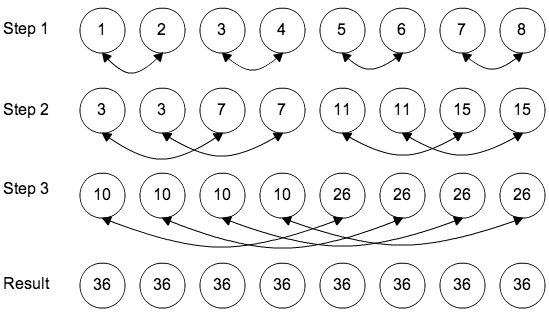
\includegraphics{recursive-doubling}
    \caption{Recursive Doubling Algorithm}%
    \label{fig:recursive-doubling}
\end{figure}

Several algorithms to realize the Allreduce operation have been
proposed~\autocite{Rabenseifner2004,Thakur2005,Kandalla2012,Ruefenacht2017}.
This research focuses on \emph{recursive doubling}~\autocite{Thakur2005},
since it requires more inter-node communication compared with other
algorithms, which means more room for optimization in terms of communication.
Figure~\ref{fig:recursive-doubling} illustrates how the recursive doubling
algorithm works. The recursive doubling algorithm requires $\log p$
communication steps where $p$ denotes the number of processes. For explanatory
purposes, the \emph{distance} between two MPI processes is defined as the
absolute difference of their rank numbers here. In the first step, processes
that are one distance apart exchange their data and perform the reduction
operation between the data that the process has originally held and with the
just exchanged data. In the second step, processes that are 2 distance apart
exchange their data, and in the $i$-th step, processes that are $2^{i - 1}$
distance apart exchange their data. The SDN MPI library memorizes all process
pairs that have to communicate and exchange data by following each step of the
recursive doubling algorithm. For each of those pairs, the library notifies
the SDN controller to prepare each route.

\section{Evaluation}\label{sec:iii-evaluation}

\subsection{Experimental Environment}

An experiment was conducted to compare the execution time of MPI\_Allreduce
accelerated with the proposed framework against conventional
MPI\_Allreduce. The experimental environment is illustrated in
Fig.~\ref{fig:experiment-environment}. This experiment was performed on
a real cluster system consisting of 28 compute nodes and 6 SDN-enabled
switches, which formed a two-tier fat-tree topology. The compute nodes and
SDN-enabled switches were all connected through Gigabit Ethernet links;
hence the interconnect was oversubscribed.

In addition to the network connecting the compute node and switches,
another network was prepared for control and management. This network
connects compute nodes, SDN-enabled switches and the SDN controller.
The interaction between the SDN controller and SDN switches is performed
via OpenFlow protocol with this management network. The compute node
that runs MPI's rank 0 process and the SDN controller also communicates
with this network. Other compute nodes were connected to the
management network as well, but those connections were not used in this
experiment.

CentOS 6.4 was installed on all computers including the compute nodes and
SDN controller. The SDN controller was developed using a SDN controller
framework Trema~\autocite{trema} 0.4.6 and Ruby 1.9.3. The SDN
MPI Library and the benchmark application were written in C and
compiled with gcc 4.4.7. As a representative of a conventional MPI,
Open~MPI~\autocite{Gabriel2004} 1.5.4 was used.

\begin{figure}
    \centering
    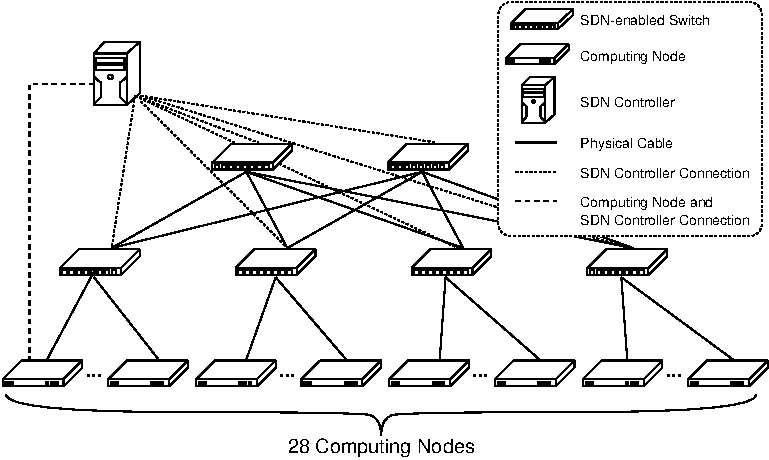
\includegraphics{sdn-mpi-exp-env}
    \caption{Experimental Environment}%
    \label{fig:experiment-environment}
\end{figure}

\subsection{Measurement Result}

A micro-benchmark that repeats MPI\_Allreduce 20
times and measures the average execution time of the function was used
for comparing the execution time of the proposed MPI\_Allreduce
with its Open~MPI counterpart.

Figure~\ref{fig:evaluation-8nodes} shows the measurement results using 8
nodes, where the horizontal axis indicates the message size and the
vertical axis shows the average time taken to execute
MPI\_Allreduce. The solid line and dashed line represent the
execution time of the proposed framework and Open~MPI implementation,
respectively. Figure~\ref{fig:evaluation-8nodes-normalized} shows the speedup
of MPI\_Allreduce accelerated using the proposed framework in comparison with
the Open~MPI implementation. The maximum of performance improvement was 41\%.

\begin{figure}
    \centering
    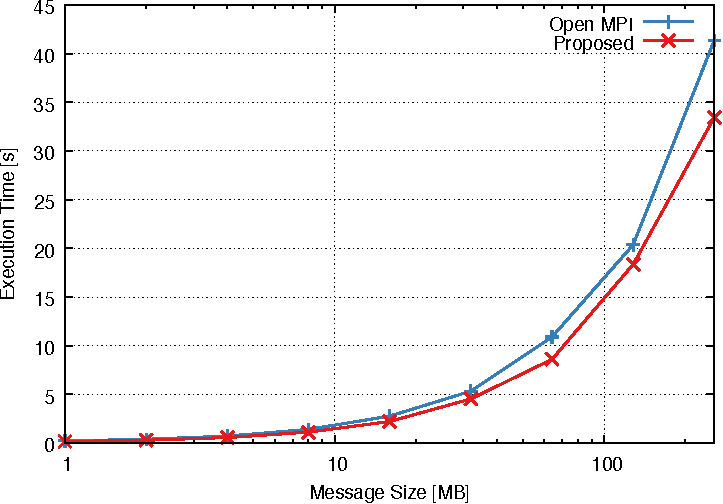
\includegraphics{allreduce_8nodes}
    \caption{Comparison of Execution Time of MPI\_Allreduce (8 Compute Nodes)}%
    \label{fig:evaluation-8nodes}
\end{figure}

\begin{figure}
    \centering
    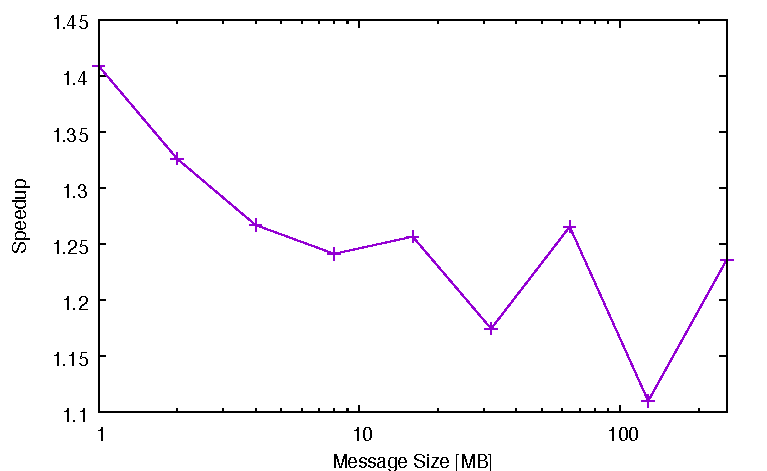
\includegraphics{allreduce_8nodes_speedup}
    \caption{Speedup of Proposed MPI\_Allreduce (8 Compute Nodes)}%
    \label{fig:evaluation-8nodes-normalized}
\end{figure}

Figure~\ref{fig:evaluation-16nodes} shows the result in the case of using 16
nodes. Figure~\ref{fig:evaluation-16nodes-normalized} indicates the speedup of
the proposed MPI\_Allreduce. It shows how the proposed framework succeeded
to reduce the execution time of MPI\_Allreduce for 56\% at most.

\begin{figure}
    \centering
    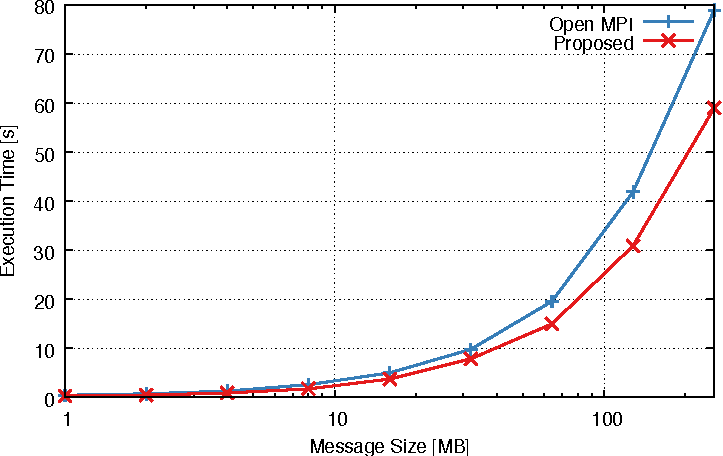
\includegraphics{allreduce_16nodes}
    \caption{Comparison of Execution Time of MPI\_Allreduce (16 Compute Nodes)}%
    \label{fig:evaluation-16nodes}
\end{figure}

\begin{figure}
    \centering
    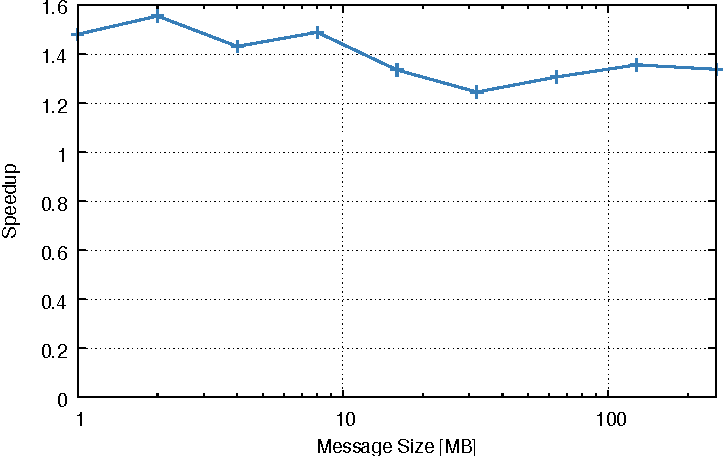
\includegraphics{allreduce_16nodes_speedup}
    \caption{Speedup of Proposed MPI\_Allreduce (16 Compute Nodes)}%
    \label{fig:evaluation-16nodes-normalized}
\end{figure}

\section{Related Work}\label{sec:iii-related-work}

There have been many research works related to MPI\@. Since MPI is merely a
specification for standard APIs for parallel programming, several algorithms
for collective operations have been proposed and implemented targeting several
network technology. As a representative example of such works,
MVAPICH~\autocite{mvapich} can be raised. MVAPICH is an MPI implementation
targeting InfiniBand, which most of high-performance computing systems ranked
in Top500 have adopted. Sur \emph{et al.}~\autocite{Sur2011} designed an MPI
library by leveraging novel InfiniBand-offered features. They explored new
architectures from a system point of view and new programming paradigms from
an application point of view to keep scaling out applications on more powerful
computing systems. Jiuxing \emph{et al.}~\autocite{Jiuxing2004} also
investigated an MPI communication protocol focusing on RDMA operations in
InfiniBand. The approach of this research has some points in common in terms
that this research also aims to benefit from the features of the underlying
network. However, this research leverages Software-Defined Networking instead
of InfiniBand from the purpose of investigating the feasibility of dynamic
control of network from an application point of view.

Researchers have attempted to elaborate algorithms for MPI collective
operations. Optimized algorithms have been proposed for
MPI\_Alltoall~\autocite{Bruck1997},
MPI\_Reduce\_scatter~\autocite{Iannello1997}, MPI\_Reduce and MPI\_Allreduce.
Most of the optimized algorithms are specialized either for latency or
throughput, so switching multiple algorithms depending on the message size or
process number makes the MPI implementation behave faster for various message
sizes and process numbers~\autocite{Thakur2005}.

Another approach is to offload the communication or computation of collective
communication operations to hardware. For example, the
\emph{K-computer}~\autocite{Yokokawa2011} has a hardware module called
\emph{Tofu Barrier Interface}~\autocite{Ajima2012} on all nodes. This module
executes Barrier, Broadcast, Reduce and Allreduce collective operations in
hardware instead of software. However, this approach does not mitigate
the congestion on links.

Past works including existing MPI implementations have been successful in
switching between multiple algorithms depending on message size, node number,
\emph{etc.} to accelerate collective communication in MPI\@. Using such a
mechanism, some estimation of the threshold value for parameters like message
size, node number, \emph{etc.} is essential. Pje\v{s}ivac-Grbovi\'{c} \emph{et
al.}~\autocite{PjesivacGrbovic2007} compared several parallel communication
models that are frequently used for dynamically estimating the threshold
values. In contrast, the current implementation of the proposed framework
always uses recursive doubling for executing MPI\_Allreduce. Therefore, the
proposed framework has a disadvantage in the cases where small data size is
treated on MPI\_Allreduce and thus the latency is more respected than the
bandwidth. For this disadvantage, automatic switching of algorithms that
leverages estimation models is planned to be introduced.

The Fabric Collective Accelerator (FCA)~\autocite{fca} is a product by
Mellanox Technologies with the target of accelerating collective
communication on clusters with InfiniBand interconnect. FCA accelerates
collective communication by offloading computations to an InfiniBand
Host Channel Adapter (HCA). It also optimizes communication flow
according to job and topology. FCA optimizes collective tree and rank
placement to control communication flow. In contrast, the proposed
framework is capable of adaptively reconfiguring the network itself,
which is more flexible. FCA also requires InfiniBand hardware, but this
research focuses on a commodity Ethernet network.

Furthermore, there have been many research reports focusing on adaptive
use of networks for high-performance computing. Geoffray \emph{et
al.}~\autocite{Geoffray2008} proposed an adaptive routing method on Myrinet
and the above-mentioned literature~\autocite{Jiuxing2004} explored the
adaptive use of multiple independent networks on InfiniBand. This research also
aims for a dynamic use of the underlying interconnection network, but differs
in the fact that this research attempted to use a different interconnection
network.

\section{Conclusion}\label{sec:iii-conclusion}

This chapter has attempted to reduce the execution time of MPI
collectives by dynamically controlling the packet flow in the interconnect
using Software-Defined Networking~(SDN).
By using SDN, this research  has proposed a novel framework for accelerating
collectives that can effectively make use of redundant routes by having SDN
interact with the communication pattern of collectives. A system of three
modules cooperating together has been designed and implemented to realize the
proposed framework. The evaluation conducted in this chapter showed that the
proposed framework speeds up the execution time of MPI\_Allreduce for 56\% at
most compared with a conventional implementation of MPI\_Allreduce. This
result confirms the superiority of the proposed framework over conventional
methods.

Several issues to tackle have remained for the realization of practical
and useful collective acceleration framework leveraging SDN\@.
The first issue is the support for multiple processes on a single compute
node. On modern computing platforms where multiple cores are implemented in a
single compute node, the assumption set in this preliminary stage of this
research is neither practical nor realistic. Therefore, intra-node
communication for pure MPI jobs needs to be considered by integrating
kernel-assisted communication such as KNEM~\autocite{Goglin2013} or Cross
Memory Attach~(CMA) with the proposed method. Also, computing paradigms such
as the hybrid use of OpenMP with MPI must be considered for enhancing
practicality. Also, other implementations of MPI such as
MVAPICH~\autocite{mvapich} are essential for investigating the practicality
and usefulness of SDN\@.

The second issue regards the necessity of additional experiments on a
larger scale environment. This chapter has verified the feasibility and
possibility of the proposed framework through the experiments using a simple
prototypical implementation. However, because OpenFlow switches were expensive
and thus only a small-scale cluster was available, only a limited number of
experiments in a small cluster environment could be conducted. Therefore,
further experiments on a larger scale environment are essential for the
evaluation of future scalability.

The third issue is the scalability issue caused by the SDN controller.
Since the current implementation requires communication between MPI processes
and SDN controller and route generation for each MPI communication request,
the SDN controller might become a scalability bottleneck on larger
environments. Therefore, the IP address and MPI rank number for each process
need be cached in the SDN controller. Furthermore, the current implementation
needs to be enhanced so that only the root process interacts with the SDN
controller and conveys information of all participating processes in the
collective communication.

\chapter{Coordination Mechanism of Communication and Computation}\label{sec:iv}

\section{Introduction}\label{sec:iv-introduction}

Recent scientific research has been taking major advantage of
computational analysis and simulation. Sustained growth in the volume of
data generated by scientific experiments has lead to a rise in the
importance of data-intensive computing. For example, approximately 15PB
of experimental data is annually generated and processed at the Large
Hadron Collider (LHC), an experimental facility for high energy
physics~\autocite{Bird2011}.

Today, in general, data-intensive computations are performed on
high-performance computer clusters. A computer cluster is composed of a
set of compute nodes connected to a high-performance network, usually
referred to as an \emph{interconnect}. Applications designed to run on
computer clusters are based on a parallel distributed processing model.
In this processing model, a large computation is decomposed into smaller
fractions of computation and is then performed by processes running in
parallel. These processes communicate with each other for data exchange
and synchronization. For this reason, the inter-node communication
performance among processes can significantly impact the total
performance of data-intensive applications. Recent advancements of high
performance computing has heavily relied upon the high degree of
parallelism rather than the improvement of CPU clock speed.
Consequently, the total number of processes and compute nodes involved
in a computation has kept increasing. As a result, communication between
distributed processes is becoming the principal bottleneck of
data-intensive applications.

Each application running on a computer cluster has a distinct pattern of
communication among processes~\autocite{Kamil2010}. These communication
patterns are difficult to predict precisely in prior to the execution of
the application. Furthermore, most of the current interconnects
available have adopted static network control and thus are unable to
adaptively reconfigure themselves to match requirements from
applications. In fact, in InfiniBand~\autocite{Buyya2009}, which is
a currently dominant interconnect technology, the forwarding tables on
switches are usually pre-configured and remain unchanged until hardware
failure or topology change occurs.

Furthermore, current interconnects are designed to be over-provisioned
in order to satisfy the communication performance requirements of
various applications with diverse communication patterns. Such
over-provisioned interconnects are designed and provided with sufficient
network resources (\emph{e.g.} bandwidth) to minimize the overload of
interconnect such as congestion.

However, recent scale-out in the number of compute nodes has revealed
two potential shortcomings of over-provisioned designs. First, the cost
of building interconnects has become increasingly higher, which makes it
difficult to implement over-provisioned designs. This increased cost is
because of the scale and complexity of interconnects that grow
superlinearly as the number of compute nodes increases. The second
shortcoming is the underutilization of interconnects. A discrepancy
between the performance characteristics of the over-provisioned
interconnect and the aggregated network requirements of the applications
may cause some portion of the interconnect not being fully utilized.

Based on these considerations, we believe that a novel cluster
architecture which dynamically controls the packet flow in the
interconnect based on the communication pattern of the application can
alleviate the aforementioned two shortcomings of conventional
over-provisioned designs. For this reason, Software-Defined Networking
enhanced Message Passing Interface (\emph{SDN-enhanced MPI}), which is
an unconventional MPI framework that incorporates flexible network
controllability of SDN into interconnects, was proposed in our past
research. Furthermore, in past research towards SDN-enhanced MPI, we
have demonstrated that the acceleration of collective MPI communication
is feasible.

However, a technical challenge still remained in this research; namely,
applying our research achievements to real-world MPI applications. In
the preliminary stage of our current research so far, we focused on
verifying the feasibility of our idea by investigating whether
individual MPI collective communications could be accelerated or not.
Therefore, how MPI communication accelerated with SDN could be
synchronized with the execution of an MPI application remained a
question that required a new technical innovation.

To this end, we propose \emph{UnisonFlow}, a mechanism for SDN-enhanced
MPI to perform network control in synchronization with the execution of
an MPI application, based on the strategy shown
in~\autocite{Takahashi2015}. The synchronization does not incur a large
overhead so it avoids performance degradation of the applications.
Furthermore, the proposed mechanism is designed to work on actual
hardware OpenFlow switches, and is not limited to software switches or
specialized hardware.

The main contributions of this chapter are summarized as follows:

\begin{itemize}
\item
  UnisonFlow, a software-defined coordination mechanism of network
  control and execution of an MPI application is proposed.
\item
  A low-overhead implementation of the proposed concept that works on
  actual hardware OpenFlow switches is presented.
\item
  An experiment is carried out to verify whether the interconnect
  control is successfully performed in synchronization with the
  execution of an application.
\item
  A performance measurement of point-to-point communication is conducted
  to evaluate the overhead incurred by the proposed mechanism.
\end{itemize}

The remainder of this chapter is organized as follows.
Section~\ref{sec:iv-objective} introduces SDN-enhanced MPI and its key
technologies. Subsequently, the challenge to realize SDN-enhanced MPI is
derived. Section~\ref{sec:iv-proposal} describes our proposed mechanism and its
implementation. Section~\ref{sec:iv-evaluation} shows the result of the experiments
conducted to demonstrate the feasibility of the proposal.
Section~\ref{sec:iv-related-work} reviews related literature and clarifies the
contributions of this chapter. Finally, Section~\ref{sec:iv-conclusion} discusses
future issues to be tackled and concludes this chapter.

\section{Research Objective}\label{sec:iv-objective}

This section first briefly describes the two key technologies of
SDN-enhanced MPI:\@ the Message Passing Interface (MPI) and Software
Defined Networking (SDN). After outlining the current development status
of SDN-enhanced MPI, the central challenge in realizing a practical
SDN-enhanced MPI is clarified.

\subsection{SDN-enhanced MPI}\label{sec:iv-sdn-mpi}

The basic idea of SDN-enhanced MPI is to incorporate the flexible
network controllability of SDN into MPI\@. As described in
Section~\ref{sec:i-mpi}, MPI mainly focuses on hiding the
complexity of the underlying network architecture. Therefore, MPI does not
provide any functionality for explicitly controlling the network. Integrating
SDN into MPI could complement such lack of a network control feature in MPI
and allow MPI to optimize the packet flow in the network in accordance with
the communication pattern of applications.

At the time of writing this paper, we have applied the above described
basic idea to two collective MPI primitives, MPI\_Bcast and
MPI\_Allreduce as proof of concept. Experiments conducted on a real
computer cluster comprising bare metal servers and hardware OpenFlow
switches have demonstrated that the execution time of these primitives
has been successfully reduced~\autocites{Dashdavaa2013}{Takahashi2014}.
SDN-enhanced MPI\_Bcast~\autocite{Dashdavaa2013} accelerates MPI\_Bcast
by utilizing the hardware multicast functionality of OpenFlow switches.
SDN-enhanced MPI\_Allreduce~\autocite{Takahashi2014} dynamically
reconfigures the path allocation based on the communication pattern of
MPI\_Allreduce so that congestion in links is minimized.

\subsection{Central Challenge of SDN-enhanced MPI}

The central challenge in realizing a practical SDN-enhanced MPI lies in
a coordination mechanism between the application and network control.
Although the previous works on SDN-enhanced MPI have shown the
feasibility of accelerating individual primitives as described in
Section~\ref{sec:iv-sdn-mpi}, actual MPI applications have not yet
taken advantage of network programmability brought by SDN, since each of
the distinct network control algorithms designed for an MPI primitive
cannot be activated along with the execution of an MPI application. In
other words, no mechanism exists that conveys the type and option of the
MPI primitive being executed at the moment by an application to the
network controller in charge of acceleration of the corresponding
primitive.

In this chapter, we realize a software-defined coordination mechanism to
perform network control in synchronization with the execution of an
application. Furthermore, the following technical requirements must be
met by the mechanism:

\begin{itemize}
\item
  \emph{Low overhead}: The overhead incurred by the proposed coordination
  mechanism should not degrade the communication performance of MPI, since the
  final goal is to improve the total performance of the MPI application.
\item
  \emph{Interoperability with hardware OpenFlow switches}: We place emphasis
  on developing a practical implementation that works on computer clusters.
  Therefore, the mechanism should work on actual hardware OpenFlow switches,
  and should not be limited to software switches or specialized hardware.
\item
  \emph{Compatibility with existing MPI library}: To mitigate the
  cost to port existent MPI applications on SDN-enhanced MPI, the existent MPI
  application should work on SDN-enhanced MPI without the source code being
  modified or recompiled. Compatibility with existing MPI implementations is
  essential for the portability of applications.
\end{itemize}

\section{Proposal}\label{sec:iv-proposal}

\subsection{Basic Idea}\label{sec:iv-basic-idea}

The basic idea of UnisonFlow is to embed MPI context information as a
\emph{tag} into each packet released through the MPI library and handle
packets based on their tags in switches. The tag is stored in the header
field of each packet. In this paper, MPI context information is defined
as a collection of application-aware data which identifies an
communication of an MPI communication primitive. Specifically, an MPI
primitive type, source/destination rank and communicator constitute MPI
context information.

A straightforward approach to realize application-aware network control
is to enhance the packet processing feature of OpenFlow switches in a
way that switches can read application-layer information from packets
and then make decisions based on that information. However, this
approach requires significant alteration to the switch hardware itself
and the OpenFlow protocol, because packet processing on switches is
mostly performed on fixed dedicated hardware components. The proposed
mechanism stores application-layer information into a header field of
packets so that OpenFlow switches can perform application-aware packet
flow control.

In detail, the tag is embedded into the destination MAC address field of
the packet header field. The location of the destination MAC address
field in a packet and the binary layout of a tag are shown in
Fig.~\ref{fig:binary-layout}.

\begin{figure}
    \centering
    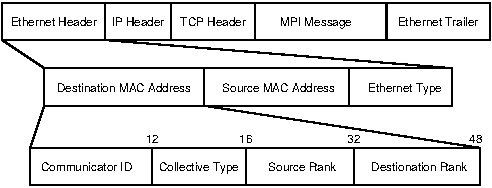
\includegraphics[width=0.8\linewidth]{binary-layout}
    \caption{Tag Information Embedded in a Packet}%
    \label{fig:binary-layout}
\end{figure}

Two main reasons exist for using the destination MAC address header
field. The first reason is that the MAC address is defined as one of the
header fields that can be used as a matching condition in OpenFlow. For
this reason, there is no need to extend or modify existing OpenFlow
switches to support this header field. The second reason is explained
from the advantage in the number of installable flow entries. Although
there are header fields other than the destination MAC address that can
be used as a matching condition in OpenFlow, switches are typically
equipped with a special hardware dedicated for L2 header field lookups.
As a result, more flow entries that include only L2 header fields can be
stored than the flow entries with other header fields.

\subsection{Architecture}

\subsubsection{Overview}

Figure~\ref{fig:overall-arch} illustrates an overview of UnisonFlow. At
this stage of research, it is assumed that a computer cluster executes a
single MPI application because our research target is the acceleration
of inter-node communication in MPI\@. The operating system of compute
nodes is assumed to be Linux.

\begin{figure}
    \centering
    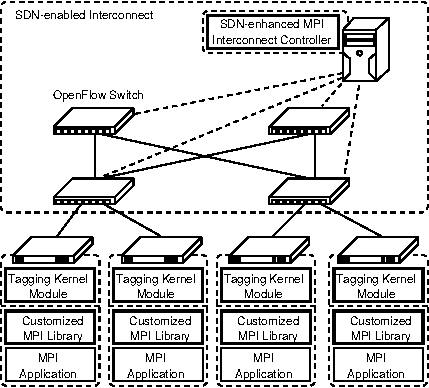
\includegraphics[width=0.7\linewidth]{overall-arch}
    \caption{Overall Architecture of UnisonFlow}%
    \label{fig:overall-arch}
\end{figure}

We have developed three major software modules that constitute this
architecture (bold rectangles in Fig.~\ref{fig:overall-arch}). The first
module is the \emph{Interconnect Controller}, which is basically an
OpenFlow controller responsible for installing flow entries into
OpenFlow switches. The interconnect controller was developed based on
the Ryu SDN controller framework~\autocite{Ryu2014}. The second module
is the \emph{Tagging Kernel Module}. It resides in the kernel space of
each compute node. The role of the tagging kernel module is to extract
MPI context information from each packet emitted by the MPI library,
encode this context information as a tag and then apply it to the
packet. The third module is the \emph{Customized MPI Library,} which is
dynamically linked to the MPI application. MPICH~\autocite{Gropp2002},
an implementation of MPI, was extended so that it meets our needs.
Specifically, it was enhanced to communicate with the tagging kernel
module and to send active connection information to the kernel module.

\subsubsection{Intra-node architecture}

On each compute node, the tagging kernel module and MPI library work
together to embed MPI context information as a tag into each packet. The
kernel module performs the actual tagging procedure, whereas the MPI
library provides the kernel module with supplementary information used
for filtering out non-MPI traffic.

As described in Section~\ref{sec:iv-basic-idea}, UnisonFlow exploits the
destination MAC address field of a packet as a place to store the
corresponding tag. To implement this, a functional component that
dynamically rewrites MAC address fields of packets is essential.

As a possible solution for the functional component on the Linux kernel,
we have considered \emph{ebtables}, \emph{raw socket} and \emph{protocol
handler}~\autocite{Rosen2013}. Ebtables is a widely adopted L2 packet filter
implemented on top of the netfilter framework. It mainly features L2 packet
filtering and Network Address Translation~(NAT). Raw sockets are special type
of sockets that give user space programs access to the whole packet including
protocol headers. TCP/UDP sockets only allows users space programs to read or
write TCP/UDP payloads, whereas raw sockets allows programs to read and write
TCP/UDP, IP and Ethernet protocol headers. In return, the user space program
has the full responsibility to handle the network protocol correctly. The
network stack of Linux kernel is designed to be extensible so that new network
protocols can be added relatively easily. New protocols can be implemented
as a protocol handler, which is essentially a call back function that is
invoked when a packet is sent or received. When implemented in a loadable
kernel module, protocol handlers can be added without recompiling the kernel.

Out of these potential solutions,
we have adopted the protocol handler because it achieves both
flexibility in rewriting of the packets depending on their payload and
minimal alteration to the MPI library. As previously described, ebtables
has a MAC NAT feature; however, it has a limitation where the MAC
addresses can only be translated to pre-configured addresses. On the
other hand, the use of a raw socket results in an extensive modification
of the MPI library, since it requires the MPI library to handle the
TCP/IP stack. In contrast to these two methods, the use of the protocol
handler facilitates the interception of packets in the network stack of
the kernel and arbitrary modifications to those packets. For this
reason, we can utilize the network stack of the kernel and avoid
re-implementing another network stack. Moreover, the whole packet
including header and payload can be read and written by the protocol
handler for dynamically rewriting the MAC address fields of packets.

Figure~\ref{fig:intra-node-flow} illustrates how MPI packets are
processed on a compute node. The solid arrows represent packet flows
generated by an MPI application. The dashed arrow represents interaction
between software modules.

\begin{figure}
    \centering
    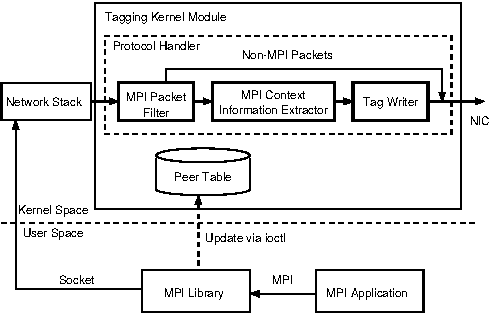
\includegraphics[width=0.8\linewidth]{intra-node-flow}
    \caption{Intra-node Packet Flow}%
    \label{fig:intra-node-flow}
\end{figure}

Once the tagging kernel module is loaded into the kernel space at the
boot time of the Linux operating system, the kernel module registers its
own protocol handler to the kernel using the
\lstinline!dev_add_pack! API\@. This protocol handler is
called every time a packet is sent out from the network stack to the
Network Interface Card (NIC). Intercepted packets sequentially undergo
three major phases of packet processing, which are performed by the
following three components (bold rectangles in
Fig.~\ref{fig:intra-node-flow}), respectively:

\begin{enumerate}
\def\labelenumi{\arabic{enumi}.}
\item
  \emph{MPI packet filter}: Packets generated by SSH, remote file
  systems, and any programs other than MPI are immediately forwarded to
  the NIC\@. To investigate whether a packet originates from MPI or not,
  this component looks up the \emph{peer table} maintained by the
  tagging kernel module and verifies if the packet is a part of the TCP
  connections opened by the MPI library. The peer table is designed as a
  hash table of all TCP connections to other processes opened by MPI\@.
  The 4-tuple (source IP, destination IP, source port and destination
  port) of each packet is used to identify a TCP connection.
\item
  \emph{MPI context information extractor}: This component extracts the
  MPI context information from packets by reading and parsing their
  message envelope. The message envelope is essentially a header that is
  prepended to every MPI message by the MPI library for identification.
  Although the message envelope is prescribed in the MPI
  specification~\autocite{MessagePassingInterfaceForum2015}, its actual binary
  layout is implementation dependent.
\item
  \emph{Tag writer}: This component encodes the context information
  extracted in the previous phase as a virtual MAC address and writes it
  into the packet. The virtual MAC address is generated by packing the
  components of MPI context information into the binary format shown in
  Fig.~\ref{fig:binary-layout}. Technically, the MAC addresses of
  packets can be modified by simply overwriting the specific position of
  the \lstinline!sk_buff! structure, which is the
  internal representation of network packets in the kernel.
\end{enumerate}

As described, the tagging kernel module maintains the peer table to keep
track of all connections opened by the locally-running MPI process to
other MPI processes running on remote compute nodes. In order to
update the content of the peer table in accordance with the internal
information of the MPI library, the MPI library has been enhanced to
provide this information to the kernel module. As the communication
channel between the MPI library and kernel module, the
\lstinline!ioctl! system call has been leveraged. These
modifications have been made so that functional compatibility with the
original MPI library was guaranteed.

\subsubsection{Inter-node architecture}

Switches composing the interconnect forward packets based on their tag
value. These forwarding rules are stored in the form of flow entries and
managed by the centralized interconnect controller.

The decision about how a packet is forwarded is made by the \emph{MPI
primitive module}, which is a pluggable software component integrated
into the interconnect controller. A unified interface between the MPI
primitive module and the interconnect controller is defined for
simplified development and integration of primitive modules. Each MPI
primitive module is expected to be designed dedicatedly for a single
type of MPI primitive.

Figure~\ref{fig:inter-node-flow} illustrates an example of the packet
flow between two remote compute nodes. When the interconnect
controller receives a packet-in message caused by an unmatched packet
(step 1 in Fig.~\ref{fig:inter-node-flow}), the controller decodes the
tag embedded in the packet and extracts the MPI context information
(step 2). After that, the responsible MPI primitive module is invoked
with the context information as its input (step 3). The MPI primitive
module determines how a set of packets carrying the same context
information should be treated. Based on this decision, flow entries are
generated and then installed to relevant switches (step 4).

\begin{figure}
    \centering
    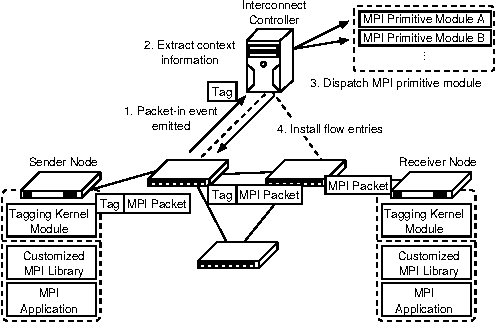
\includegraphics[width=0.8\linewidth]{inter-node-flow}
    \caption{Inter-node Packet Flow}%
    \label{fig:inter-node-flow}
\end{figure}

Note that NICs drop incoming packets whose destination addresses are not
the address of NICs unless they are put into promiscuous mode.
Therefore, the destination MAC address of tagged packets needs to be
restored to the true MAC address of its receiver node. This restoration
is achieved by appending an action for changing the MAC address field to
the flow entry installed on the switch adjacent to the receiver node.

\section{Evaluation}\label{sec:iv-evaluation}

Two experiments were conducted to examine the feasibility of UnisonFlow.
In the first experiment, the control of the interconnect is investigated
in terms of whether it is properly synchronized with the execution of
the application. In the second experiment, the overhead imposed by
UnisonFlow is evaluated.

\subsection{Experimental environment}

Both of the two experiments were conducted on the SDN-enabled computer
cluster shown in Fig.~\ref{fig:cluster-topology}. For the topology of
the interconnect, a two-tier fat-tree composed of six switches was
adopted because fat-trees are one of the most widely used topologies for
today's cluster systems. Note that each of the two physical switches was
divided to three logical switches due to a limited number of available
OpenFlow switches in our institution. In the following discussion, we
refer to the two upper layer switches as spine1 and spine2, whereas the
four lower layer switches are referred to as leaf1, leaf2, leaf3 and
leaf4, respectively. Spine switches and leaf switches were connected on
4 Gbps links, each of which was an aggregated link of four GbE links.
Six compute nodes were connected to a leaf switch; that is, 24
compute nodes in total. These compute nodes are hereinafter referred
to as node01 to node24. Leaf switches and compute nodes were
interconnected with 1Gbps Ethernet. A management node accommodating the
interconnect controller was also prepared.

\begin{figure}
    \centering
    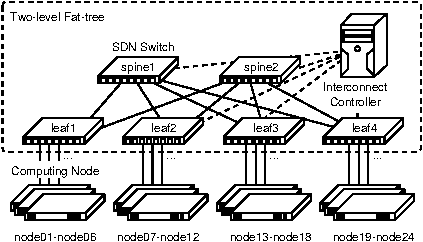
\includegraphics[width=0.8\linewidth]{cluster-topology}
    \caption{Overview of the Experimental Environment}%
    \label{fig:cluster-topology}
\end{figure}

For SDN switches, NEC ProgrammableFlow PF5240 has been adopted. The ompute
node was a SGI Rackable Half-Depth Server C1001 equipped with the hardware and
software as shown in Table~\ref{tbl:node-spec}.

\begin{table}
    \centering
    \caption{compute node Specifications}%
    \label{tbl:node-spec}
    \begin{tabular}{ll}
        \toprule
        Name        & Spec                                        \\ \midrule
        CPU         & Intel Xeon E5-2620 2.00GHz 6core $\times$ 2 \\
        Memory      & 64GB (DDR3-1600 8GB $\times$ 8)             \\
        Network     & Gigabit Ethernet                            \\
        OS          & CentOS 7.2                                  \\
        Kernel      & Linux 3.10                                  \\
        MPI Library & MPICH 3.1.4                                 \\ \bottomrule
    \end{tabular}
\end{table}

\subsection{Verification of coordination mechanism}

The first experiment was conducted to verify whether the dynamic control
of packet flows on the interconnect was performed in synchronization
with the execution of the application. To verify the synchronization
between interconnect control and execution of the application, an MPI
application which sequentially executes two different MPI primitives has
been developed. The interconnect controller applies different routing
strategies for each primitive as MPI primitive modules. We then observe
the packet flow on the interconnect using the port counters of switches
to verify if the interconnect control can successfully switch from one
to another when the MPI primitive executed changes.

The detailed experimental setup is as follows. The MPI application
executes an iteration of MPI\_Bcast followed by another iteration of
MPI\_Reduce. List~\ref{lst:sync-mpi-app} shows a simplified source code
of this application. The process with rank 0 is specified as the root
process for both MPI\_Bcast and MPI\_Reduce. The rank 0 process is
configured to run on node01, which is connected to switch leaf1.
Furthermore, the MPI application records the time where each of the
following three events occurs: the start of the MPI\_Bcast iteration
(\(t_1\)), the start of the MPI\_Reduce iteration (\(t_2\)) and the
finish of the MPI\_Reduce iteration (\(t_3\)). This timing information
is used to investigate the relationship between the execution of the MPI
application and the traffic change in the interconnect.

\begin{figure}
    \centering
    \begin{subfigure}{.45\linewidth}
        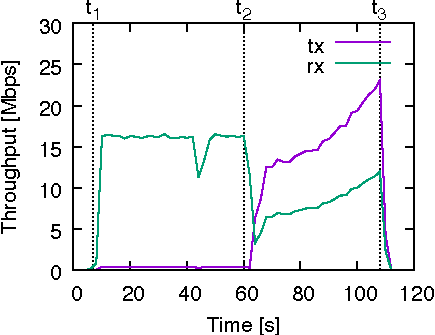
\includegraphics[width=.95\linewidth]{coll-conv-1-2560}
        \caption{At Port 0xa00 (spine1) \newline Towards Port 0xa00 (leaf1)}%
        \label{fig:spine1-leaf1-conv}
    \end{subfigure}
    \begin{subfigure}{.45\linewidth}
        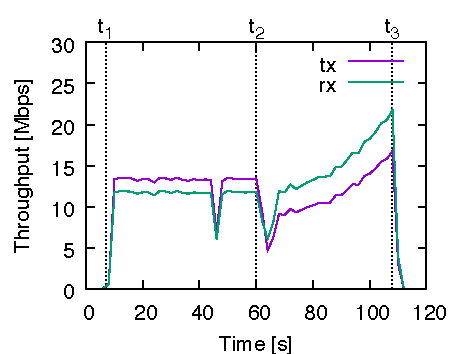
\includegraphics[width=.95\linewidth]{coll-conv-1-2816}
        \caption{At Port 0xb00 (spine1) \newline Towards Port 0xa00 (leaf2)}%
        \label{fig:spine1-leaf2-conv}
    \end{subfigure}
    \begin{subfigure}{.45\linewidth}
        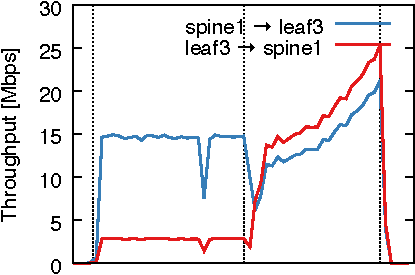
\includegraphics[width=.95\linewidth]{coll-conv-1-3072}
        \caption{At Port 0xc00 (spine1) \newline Towards Port 0xa00 (leaf3)}%
        \label{fig:spine1-leaf3-conv}
    \end{subfigure}
    \begin{subfigure}{.45\linewidth}
        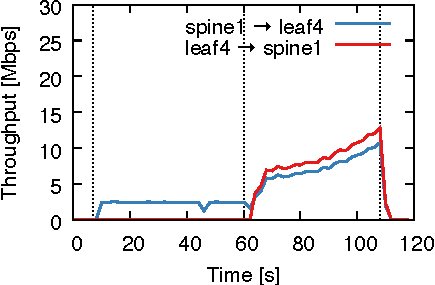
\includegraphics[width=.95\linewidth]{coll-conv-1-3328}
        \caption{At Port 0xd00 (spine1) \newline Towards Port 0xa00 (leaf4)}%
        \label{fig:spine1-leaf4-conv}
    \end{subfigure}
    \caption{Throughput Measured at Ports on Switch spine1 (conventional)}%
    \label{fig:coll-spine1-conv}
\end{figure}

\begin{figure}
    \begin{subfigure}{.45\linewidth}
        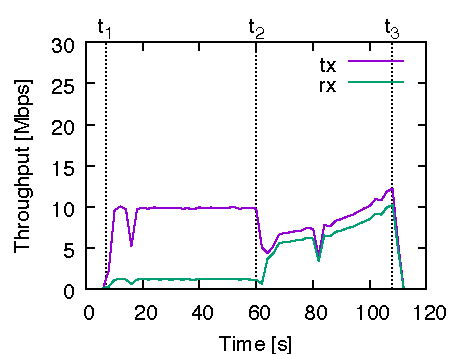
\includegraphics[width=.95\linewidth]{coll-conv-2-2560}
        \caption{At Port 0xa00 (spine2) \newline Towards Port 0xa00 (leaf1)}%
        \label{fig:spine2-leaf1-conv}
    \end{subfigure}
    \begin{subfigure}{.45\linewidth}
        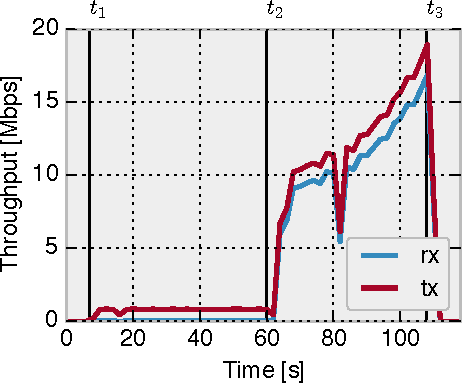
\includegraphics[width=.95\linewidth]{coll-conv-2-2816}
        \caption{At Port 0xb00 (spine2) \newline Towards Port 0xa00 (leaf2)}%
        \label{fig:spine2-leaf2-conv}
    \end{subfigure}
    \begin{subfigure}{.45\linewidth}
        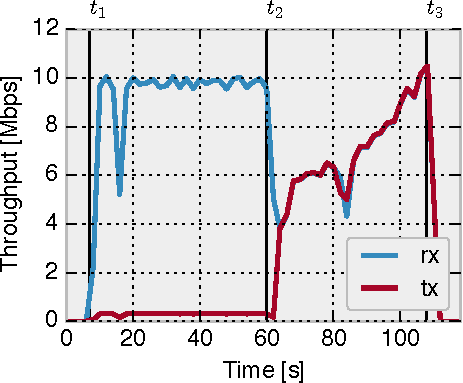
\includegraphics[width=.95\linewidth]{coll-conv-2-3072}
        \caption{At Port 0xc00 (spine2) \newline Towards Port 0xa00 (leaf3)}%
        \label{fig:spine2-leaf3-conv}
    \end{subfigure}
    \begin{subfigure}{.45\linewidth}
        \includegraphics[width=.95\linewidth]{coll-conv-2-3328}
        \caption{At Port 0xd00 (spine2) \newline Towards Port 0xa00 (leaf4)}%
        \label{fig:spine2-leaf4-conv}
    \end{subfigure}
    \caption{Throughput Measured at Ports on Switch spine2 (conventional)}%
    \label{fig:coll-spine2-conv}
\end{figure}

Each MPI primitive is repetitively executed because a single invocation
of these primitives completes too quickly to observe the traffic change.
The port counters of PF5240 are updated approximately once a second.
This implies that instant traffic changes happening in less than one
second cannot be precisely observed. Since a single invocation of
MPI\_Bcast or MPI\_Reduce finishes in the order of milliseconds, we
repeat each primitive to make its total execution time longer so that we
can observe the traffic change using port counters.

\begin{lstlisting}[caption={Source code of MPI application}, label=lst:sync-mpi-app, float=htbp]
#include <mpi.h>
#define BUF_SIZE     (1000)
#define REPEAT_COUNT (10000)

char send_buf[BUF_SIZE];
char recv_buf[BUF_SIZE];

int main(int argc , char** argv) {
    MPI_Init(&argc , &argv);

    /* Record current time as $t_1$ */

    /* MPI_Bcast */
    for (i = 0; i < REPEAT_COUNT; i++) {
        MPI_Bcast(send_buf, BUF_SIZE, MPI_CHAR, 0,
                  MPI_COMM_WORLD);
    }

    /* Record current time as $t_2$ */

    /* MPI_Reduce */
    for (i = 0; i < REPEAT_COUNT; i++) {
        MPI_Reduce(send_buf, recv_buf, BUF_SIZE,
                   MPI_CHAR, MPI_SUM, 0,
                   MPI_COMM_WORLD);
    }

    /* Record current time as $t_3$ */

    MPI_Finalize();
}
\end{lstlisting}

Under the interconnect topology of this experimental environment, there
are always two possible paths between any two different leaf switches.
One is the path that contains spine1 (\emph{e.g.} leaf1 - spine1 -
leaf2) and the other path contains spine2 (\emph{e.g.} leaf1 - spine2 -
leaf2). The interconnect controller was deployed with a routing strategy
that assigns paths utilizing spine1 to the traffic generated by
MPI\_Bcast. In contrast, the traffic generated by MPI\_Reduce was set so
that it goes through spine2. Note that spine switches are never utilized
by traffic between two compute nodes under an identical leaf switch.
As a representative implementation of conventional networking
architecture, an SDN controller was employed with a Equal Cost Multi
Path (ECMP) routing strategy. To observe the traffic change in the
interconnect, a measurement module that periodically (every two seconds)
gathers and reports transmitted and received bytes of every switch port
was integrated into the interconnect controller. Based on these port
counter values, we calculated the throughput of the transmitted traffic
and the received traffic of each port.

Figures~\ref{fig:coll-spine1-conv} and \ref{fig:coll-spine2-conv} show
the change of throughput observed at the ports of switches spine1 and
spine2 when using ECMP\@. Both spine1 and spine2 were utilized during the
execution of MPI\_Bcast and MPI\_Reduce as a result of load balancing.
However, there is some inequality in the utilization of two spine
switches. This inequality is because ECMP distributes the traffic
workload not on the basis of not packets, but on flows.

MPICH, which is the MPI implementation used in UnisonFlow, has optimized
implementations for collective communications like other MPI libraries.
In particular, under the environment of this experiment, MPI\_Bcast uses
binomial tree algorithm while MPI\_Reduce uses the Rabenseifner's reduce
algorithm~\autocite{Rabenseifner2004}. As a result, MPI\_Bcast is not a
simple repeated point-to-point communication from the root process to
other processes, but involves communication between non-root processes.
For instance, Fig.~\ref{fig:spine1-leaf1-conv} indicates how the traffic
between spine1 and leaf1 changes. In detail, TX shows the outgoing
traffic from spine1 to leaf1, which is the aggregated traffic from the
compute nodes under leaf2, leaf3 and leaf4 to the compute nodes
under leaf1. In contrast, RX shows the aggregated traffic from compute
nodes under leaf1 to other compute nodes under leaf2, leaf3 and leaf4.

\begin{figure}
    \centering
    \begin{subfigure}{.45\linewidth}
        \includegraphics[width=.95\linewidth]{coll-prop-1-2560}
        \caption{At Port 0xa00 (spine1) \newline Towards Port 0xa00 (leaf1)}%
        \label{fig:spine1-leaf1-prop}
    \end{subfigure}
    \begin{subfigure}{.45\linewidth}
        \includegraphics[width=.95\linewidth]{coll-prop-1-2816}
        \caption{At Port 0xb00 (spine1) \newline Towards Port 0xa00 (leaf2)}%
        \label{fig:spine1-leaf2-prop}
    \end{subfigure}
    \begin{subfigure}{.45\linewidth}
        \includegraphics[width=.95\linewidth]{coll-prop-1-3072}
        \caption{At Port 0xc00 (spine1) \newline Towards Port 0xa00 (leaf3)}%
        \label{fig:spine1-leaf3-prop}
    \end{subfigure}
    \begin{subfigure}{.45\linewidth}
        \includegraphics[width=.95\linewidth]{coll-prop-1-3328}
        \caption{At Port 0xd00 (spine1) \newline Towards Port 0xa00 (leaf4)}%
        \label{fig:spine1-leaf4-prop}
    \end{subfigure}
    \caption{Throughput Measured at Ports on Switch spine1 (proposed)}%
    \label{fig:coll-spine1-prop}
\end{figure}

\begin{figure}
    \begin{subfigure}{.45\linewidth}
        \includegraphics[width=.95\linewidth]{coll-prop-2-2560}
        \caption{At Port 0xa00 (spine2) \newline towards Port 0xa00 (leaf1)}%
        \label{fig:spine2-leaf1-prop}
    \end{subfigure}
    \begin{subfigure}{.45\linewidth}
        \includegraphics[width=.95\linewidth]{coll-prop-2-2816}
        \caption{At Port 0xb00 (spine2) \newline towards Port 0xa00 (leaf2)}%
        \label{fig:spine2-leaf2-prop}
    \end{subfigure}
    \begin{subfigure}{.45\linewidth}
        \includegraphics[width=.95\linewidth]{coll-prop-2-3072}
        \caption{At Port 0xc00 (spine2) \newline towards Port 0xa00 (leaf3)}%
        \label{fig:spine2-leaf3-prop}
    \end{subfigure}
    \begin{subfigure}{.45\linewidth}
        \includegraphics[width=.95\linewidth]{coll-prop-2-3328}
        \caption{At Port 0xd00 (spine2) \newline towards Port 0xa00 (leaf4)}%
        \label{fig:spine2-leaf4-prop}
    \end{subfigure}
    \caption{Throughput Measured at Ports on Switch spine2 (proposed)}%
    \label{fig:coll-spine2-prop}
\end{figure}


Figures~\ref{fig:coll-spine1-prop} and~\ref{fig:coll-spine2-prop} show
the change of throughput when using the proposed mechanism. In these
plots, the time of event occurrences recorded by the MPI application are
marked with vertical solid black lines. The time synchronization between
throughput change and event occurrences was made on the basis of the
timestamp. At \(t_1\) where MPI\_Bcast started, both RX and TX
throughput observed at the ports of spine1 rise steeply and then
maintain the amount of approximately 14Mbps and 9Mbps, respectively,
while there is no clear growth of throughput at the ports of spine2.
This indicates that only spine1 was utilized during the execution of
MPI\_Bcast. When MPI\_Bcast finished and then MPI\_Reduce started at
\(t_2\), a sharp fall of throughput at spine1 was observed, whereas a
rapid uptake in the throughput at spine2 was observed. After that, a
sharp drop of throughput at the ports of spine2 was observed immediately
when MPI\_Reduce finished (\(t_3\)). This measurement result indicates
that only spine2 was utilized during the execution of MPI\_Reduce. Based
on these observations, it is confirmed and verified that the network
control is synchronized with the execution of the MPI application.

\subsection{Evaluation of overhead}

\begin{figure}
    \centering
    \includegraphics[width=0.6\linewidth]{overhead-bandwidth}
    \caption{Comparison of Bandwidth}%
    \label{fig:overhead-bandwidth}
\end{figure}

\begin{figure}
    \centering
    \includegraphics[width=0.6\linewidth]{overhead-latency}
    \caption{Comparison of Latency}%
    \label{fig:overhead-latency}
\end{figure}

\begin{figure}
    \centering
    \includegraphics[width=0.6\linewidth]{overhead-latency2}
    \caption{Absolute Overhead to Latency}
    \label{fig:overhead-latency-2}
\end{figure}

The primary source of the overhead incurred by the proposed mechanism is
considered to be the tagging kernel module, because it requires
per-packet inspection and modification over all packets emitted from a
compute node. Additionally, rewriting the destination MAC address
header field in the switches to restore the true MAC address can also be
a source of overhead. In order to evaluate the total overhead caused by
the proposal, we measured the communication performance of
point-to-point MPI primitives using the OSU Micro-Benchmark Suite
5.3~\autocite{omb} between node01 and node02 and
compared the result with and without the proposed mechanism. The reason
to measure the performance of point-to-point communication and not
collective communication is to remove unwanted influence from complex
algorithms and communication patterns of collective communications. The
osu\_bw benchmark and osu\_latency benchmark included in the OSU
Micro-Benchmark suite were used to measure the bandwidth and latency,
respectively.

Figure~\ref{fig:overhead-bandwidth} shows a comparison of the throughput
observed between node01 and node02. Fig.~\ref{fig:overhead-latency}
shows the comparison result of latency for the same compute node pair.
The plots in Fig.~\ref{fig:overhead-bandwidth} and
Fig.~\ref{fig:overhead-latency} represent the average of 500
measurements and 50,000 measurements, respectively.
Fig.~\ref{fig:overhead-latency-2} shows the overhead imposed to latency
by the proposed mechanism. These plots indicate that performance
degradation imposed by the proposed mechanism is practically negligible
for both bandwidth and latency.

In this experiment, we only evaluated the performance of point-to-point
primitives. However, the fact that collective primitives are often
implemented using multiple point-to-point
primitives~\autocites{Squyres2005}{mvapich} implies that the overhead
of the proposed mechanism is negligible for collective primitives as
well.

\section{Related Work}\label{sec:iv-related-work}

Several studies~\autocites{Mekky2014}{Cheng2014} have been carried out
to incorporate application-awareness into SDN\@. An extension to Open
vSwitch and OpenFlow has been proposed~\autocite{Mekky2014} to realize
an application-aware data plane. This extension adds flow tables with
application-specific actions to the packet processing pipeline of Open
vSwitch. Although this method covers most network applications, it is
not able to efficiently read and process the payload of a packet because
the flow matching mechanism has not been modified from the plain
OpenFlow design. Thus, only pre-defined header fields can be used as
matching criteria. Moreover, applying this method to bare-metal computer
clusters is challenging because the hardware switches were out of the
focus. The packet processing pipelines of commercial hardware switches
cannot be modified since they are implemented using unmodifiable
hardware. In contrast, our research supports existing hardware switches
and per-packet inspection.

An application-aware routing scheme for big data applications has been
presented in~\autocite{Cheng2014}. This routing scheme maintains a
global view of the network topology and link usage. Based on this global
view, the network controller dynamically allocates a path for each
Hadoop network flow so that congestion is avoided and network
utilization is increased. Experiments demonstrated that the
application-aware SDN routing significantly improved the speed of the
shuffle phase in Hadoop, in comparison with conventional routing
mechanisms such as ECMP and Spanning Tree. The concept of optimizing the
packet flow in the interconnect based on application-layer information
is similar to SDN-enhanced MPI\@. However, the scheme to synchronize flow
installation and a Hadoop job has not been clarified in this research.

Hybrid Flexibly Assignable Switch Topology (HFAST)~\autocite{Kamil2007}
interconnect architecture tailors the interconnect topology to meet the
communication requirements of different applications. This is achieved
by utilizing reconfigurable optical circuit switches to dynamically
provide the connection between packet switches. Additionally, a process
allocation algorithm optimized for HFAST architecture is also presented.
HFAST architecture can reduce required hardware resources compared to
conventional fat-tree interconnects. Our research is different from this
research in terms that a technical design to extract communication
patterns from applications and convey such information to the network
controller in real-time is exhibited.

A software-defined multicasting mechanism for MPI has been presented
in~\autocite{Arap2014}. This mechanism offloads collective MPI primitives to
programmable NICs and OpenFlow switches. This method heavily depends on
specialized hardware such as NetFPGA, whereas our proposal is software-based.

Multi-Protocol Label Switching~(MPLS) and UnisonFlow share the similar
idea of eliminating the need to examine packet payloads by encoding
upper layer information into fixed-length tags that are processable by
hardware. However, to the best of our knowledge, no work has tackled to
integrate MPI with label switching networks.

\section{Conclusion}\label{sec:iv-conclusion}

In this chapter, we have proposed UnisonFlow, a software-defined
coordination mechanism for SDN-enhanced MPI that performs network
control in synchronization with the execution of an application. The
proposed mechanism is characterized by a kernel-assisted approach to tag
packets that are emitted from compute nodes with the MPI context
information of each packet. Experiments conducted on a computer cluster
have verified the synchronization between network control and the
execution of the application. Moreover, evaluation experiments have
indicated that the overhead incurred by the coordination mechanism is
practically negligible.

There are still issues to be addressed in the future. First,
SDN-enhanced MPI primitives developed in our previous
work~\autocites{Dashdavaa2013}{Takahashi2014} need to be adjusted as MPI
primitive modules on the interconnect controller and tested to see if
they are accelerated compared to conventional MPI primitives. Second,
performance evaluation using real-world MPI applications is necessary.
Although we have developed some individual SDN-enhanced MPI primitives
and UnisonFlow as the coordination mechanism of message-passing
communication and computation, it is still unclear how these elements
can accelerate a practical application as a whole. Finally, we need to
investigate how this architecture can be adopted to a computer cluster
simultaneously running multiple jobs, which is common in practical
deployments. Since our current implementation of the UnisonFlow assumes
only one job running at the same time on a node, we need to enhance it
to support multiple concurrent jobs. This enhancement might involve an
integration with the job scheduler.

\chapter{Conclusion}

\section{Concluding Remarks}

\section{Future Directions}

\chapter*{Acknoledgements}

First and foremost, I would like to express my sincere gratitude to my
supervisor Professor Shinji Shimojo. Professor Shimojo continuosly
convincingly conveyed a spirit of adventure and excitement to this study. His
excellent advices based on his deep knowledge always provided a unique
perspective and new meaning to this study.

Sincere thanks also goes to Professor Takahiro Hara, Professor Toru Fujiwara,
Professor Makoto Onizuka, Professor Yasuyuki Matsushita and Professor Norihiro
Hagita at Department of Multimedia Engineering, Graduate School of Information
Science and Technology, Osaka University for their appropriate guidance.

I would like to express my deepest appreciation to Associate Professor Susumu
Date at Cybermedia Center, Osaka University, for his patient and enthusiastic
guidance along my studies. His exceptional ability to analyze, solve and
present scientific problems has constantly impressed me. Without his support
and encouragement, this disseration would not have been possible.

I also would like to thank Associate Professor Yoshiyuki Kido and Associate
Professor Kazuhide Kojima at Cybermedia Center, Osaka University, for their
their encouragement, insightful comments, and hard questions.

This study greatly benefited from the comments and advices from Professor
Kaname Harumoto at Osaka University Institute for Datability Science,
Associate Professor Hiroki Kashiwazaki at Cybermedia Center, Osaka University,
Dr.~Eiji Kawai at National Institute of Information and Communications
Technology, Associate Professor Kohei Ichikawa at Nara Institute of Science
and Technology, Associate Professor Hirotake Abe at University of Tsukuba,
Assistant Professor Yasuhiro Watashiba at Cybermedia Center, Osaka University
and Dr.~Hiroaki Yamanaka at National Institute of Information and
Communications Technology. Their suggestions improved the quality of this
thesis much further.

I would like to thank all the students at Shimojo laboratory for the sleepless
nights we worked together before deadlines, and for all the fun we had. It was
a great pleasure working with you.

I would like express my hearfelt gratitude to my parents, Toshihito Takahashi
and Naoko Takahashi, for their continuous support, encourgement and care. They
made me the person who I am today.

Finally, but most importantly, I would like to express my deepest gratitude
and appreciation to my wife Ziyan Xu for her unconditional love and support
throughout my studies and my personal life.


\printbibliography[heading=bibintoc,title={References}]

\end{document}
